\chapter{Il ROC prototipo RD53A}
\label{cap:RD53A}

Lo sviluppo di un sistema di alimentazione seriale e, in particolare, del circuito di alimentazione ShuntLDO, che gestisce localmente le tensioni su chip, è parte integrante del ROC che viene sviluppato nell'ambito della collaborazione RD53~\cite{RD53} e, in particolare, del primo ROC prototipo messo a punto dalla collaborazione, RD53A~\cite{RD53A}, che \`e diventato disponibile per la comunit\`a scientifica alla fine del 2017.

Questo prototipo costituisce una pietra miliare molto importante per il progetto dei rivelatori a pixel per HL-LHC \`e sar\`a utilizzato non solo per validare le scelte strettamente relative al ROC stesso (resistenza alla radiazione e prestazioni rispetto ai requisiti di HL-LHC) ma anche per finalizzare lo sviluppo dei sensori e del resto dell'apparato.
%, e quindi la tolleranza al danneggiamento da radiazioni, soglie di lavoro basse e stabili nel tempo, capacità di gestire un alto flusso di particelle incidenti e l'utilizzo di trigger veloci.

\section{Organizzazione del chip, alimentazione e Front End}
\label{Organizzazionechip}


\begin{figure}
\centering
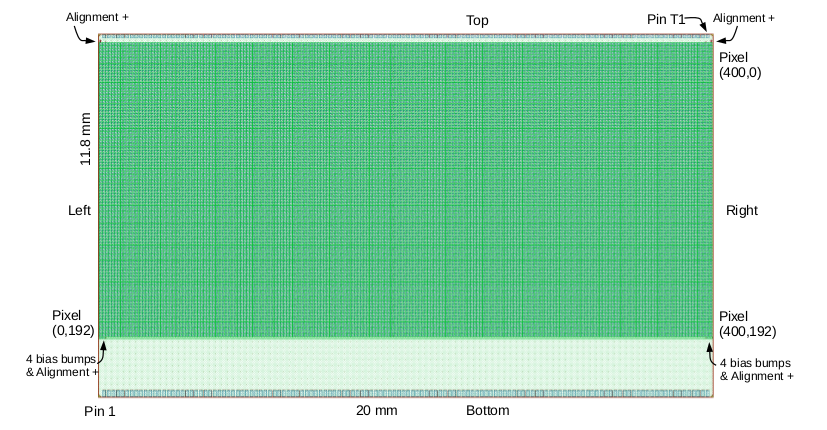
\includegraphics[scale=.4]{Immagini/RD53ALayout}
\caption{La geometria reale di RD53A: il chip è largo $20\mm \times 11.8\mm$ con una pixel matrix di $400\times 192$ pixel corrispondenti ad una area attiva di $20\mm \times 9.6\mm$.}
\label{RD53ALayout}
\end{figure}
Facendo riferimento alla Fig.~\ref{RD53ALayout}, l'area del chip che sarà saldata col sensore tramite bump bonding, detta anche {\em pixel matrix}, è posta nella parte alta ed è organizzata in una matrice di $192\times400$ pixel di area $50\um \times 50 \um$ per un'area totale di $20\mm \times 9.6\mm$.
Al di sopra di questa è presente una fila di piazzole a scopo diagnostico che saranno eliminata nella versione finale.

\begin{figure}
\centering
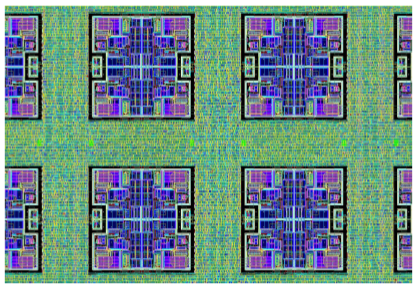
\includegraphics[scale=.5]{Immagini/AnalogIsland}
\caption{Disegno ricavato dalle maschere di RD53A dove sono visibili le `isole analogiche' dei \textit{front end} della `pixel matrix' circondate dal `mare' della circuiteria digitale.}
\label{AnalogIsland}
\end{figure} 
La matrice di pixel è organizzata in \textit{cores} di 8$\times$8 pixel, all'interno di ciascuno dei quali i 64 circuiti di preamplificzione (front end) sono disposti in regioni di 4, chiamati {\em isole analogiche}, come mostrato in Fig.~\ref{AnalogIsland}. 
Dato la miniaturizzazione necessaria, l'area del ROC deve essere completamente sfruttata e, infatti, le isole analogiche sono circondate da un `mare' di circuiteria digitale. 


\begin{figure}
\centering
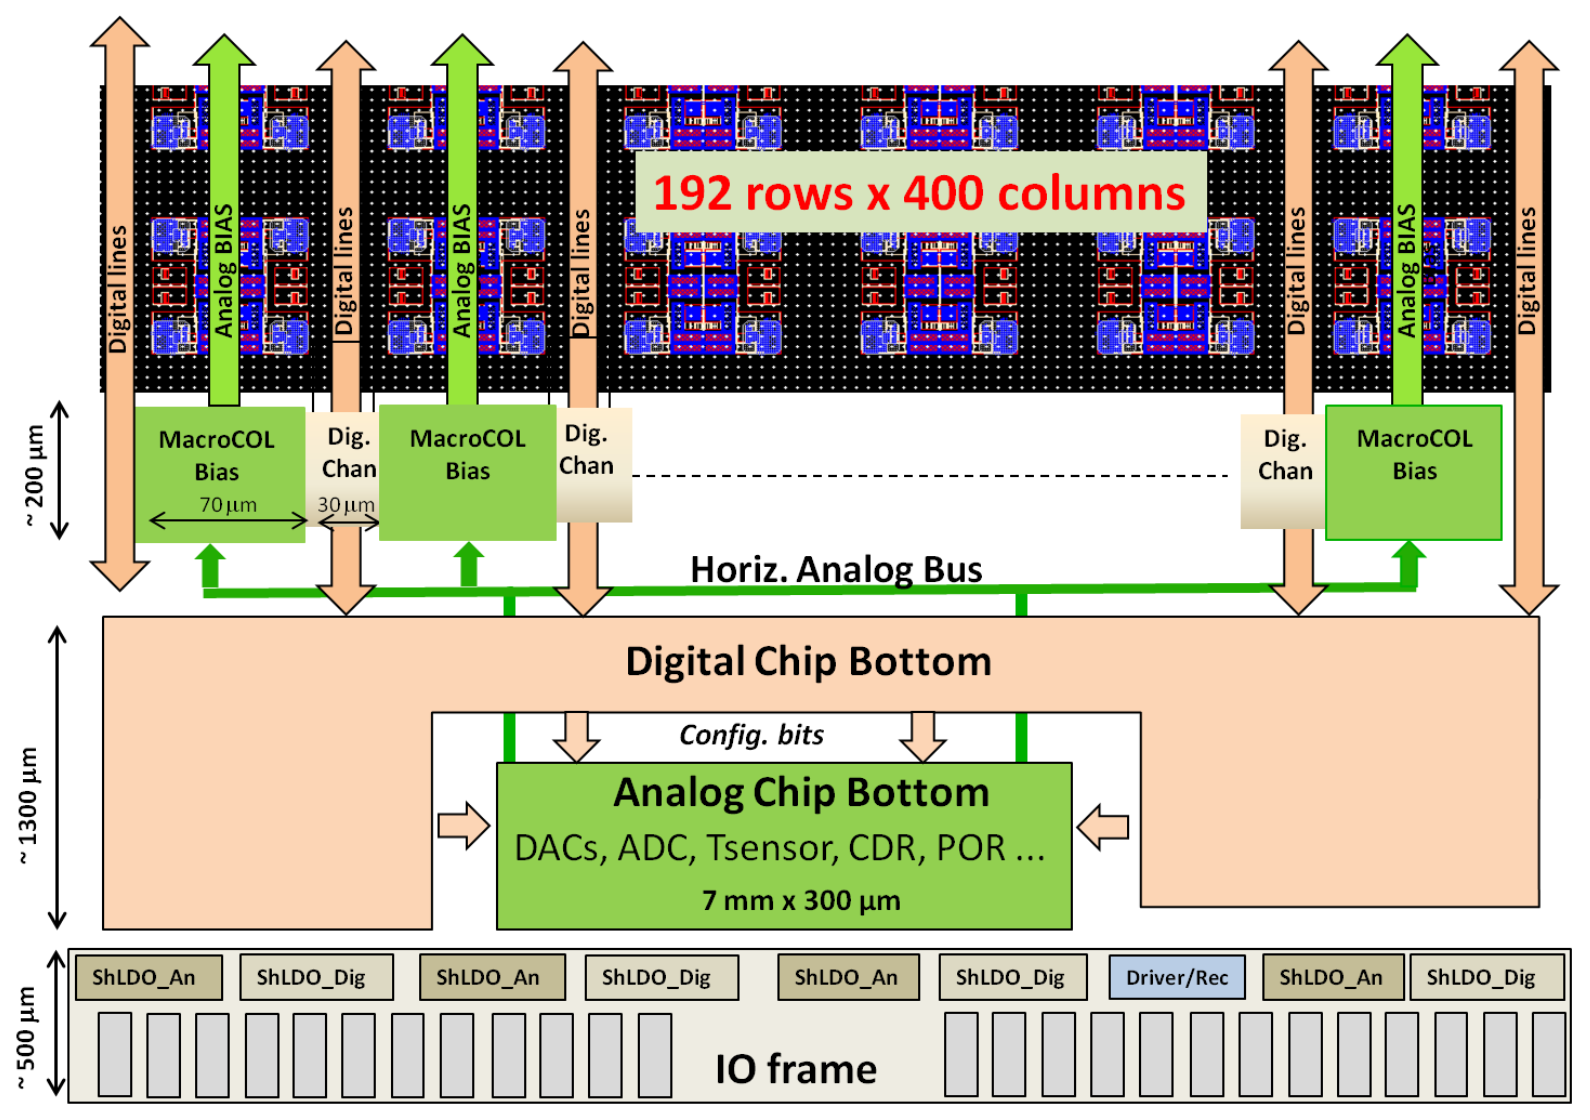
\includegraphics[scale=.4]{Immagini/RD53Apianofunzionale}
\caption{Il piano funzionale di RD53A in cui, nella parte bassa, sono visibili, in particolare, le piazzole di potenza dello ShuntLDO.}
\label{RD53AFunct}
\end{figure}
Come rappresentato nel piano funzionale in Fig.~\ref{RD53AFunct}, al di sotto delle pixel matrix \`e collocata la regione detta `periferia' che, oltre alle piazzole di microsaldatura per la connessione del ROC, ospita tutti gli altri blocchi funzionali del ROC: l'{\em Analog Chip Bottom} (ACB) ospita i blocchi analogici (DAC, ADC, sensori di temeperatura...); il {\em Digital Chip Bottom} (DCB) raggruppa i blocchi digitali per la gestione dell'Input/Output e della congigurazione. Tenendo conto della periferia la dimensione totale del chip \`e $20\mm \times 11.8\mm$.

L'alimentazione di RD53A \`e dimensionata su un numero di pixel doppio rispetto a quelli effettivamente presenti, comparabile per\`o con quello che sar\`a il ROC finale di superficie circa doppia. RD53A sar\`a normalemnte alimentato tramite un'unica linea di alimentazione seriale che serve lo ShuntLDO che fornisce VDDD (la tensione di alimentazione della parte digitale) e lo ShuntLDO che fornisce VDDA (la tensione di alimentazione della parte analogica). Essendo un prototipo \`e anche possibile alimentare direttamente le linee VDDD e VDDA scavalcando la regolazione.
Come accennato in precedenza, la parte dello ShuntLDO in cui potrebbe venire dissipata molta potenza (il mosfet di shunt M4), \`e distribuita in quattro `piazzole di potenza' per ciascun regolatore ospitate nella periferia (come visibile in~Fig.~\ref{RD53AFunct}). Solo una di queste contiene la comune parte comune di controllo dello ShuntLDO. Questo accorgimento permette di distribuire la dissipazione di calore dovuta allo shunt per una maggiore affidabilit\`a. Ciascuna piazzola \`e stata dimensionata in base al previsto consumo totale del chip finale, ovvero per una corrente massima di $500\mA$ per un totale, per tutto il ROC, tenendo conto sia della parte digitale che analogica, di $4.0\A$.

%\section{Front End}

Dato che RD53A non deve essere inteso come il prodotto finale, ma come un prototipo in cui coesistono varie possibili linee di sviluppo, al suo interno sono presenti tre differenti tipologie di circuiti di preamplificazione di front end (FE) per permettere un confronto in termini di prestazioni.
% possiede molte modifiche di design utili solo in una prima fase di test, ad esempio al suo interno sono presenti tre diversi front end (FE), già questo causa una non uniformità del chip. 
La pixel matrix \`e suddivisa equamente tra i FE Sincrono, Lineare e Differenziale come visibile in Fig.~\ref{FrontEnd}. 
%Questi tre circuiti sono stati progettati da tre differenti gruppi e tra di loro ci sono importanti differenze.

Il FE Sincrono sfrutta un sistema di \textit{auto-zeroing} della linea di base, campionandola periodicamente, invece di aggiustare la soglia pixel per pixel. 
Il FE Lineare, invece, utilizza un amplificatore lineare all'ingresso del comparatore, che confronta il segnale con la soglia impostata. 
Il FE Differenziale ha uno stadio di guadagno differenziale all'ingresso del discriminatore. % e sbilanciando i due canali implementa la soglia.

In comune ai tre FE, invece, abbiamo la rete di polarizzazione per il sensore ed il circuito per iniettare segnali di calibrazione.
%Questi ultimi due permettono un miglior confronto fra le prestazioni dei FE.
%Inoltre, i tre FE condividono l'area del sensore e, dato che la matrice è larga 400 pixel ed è suddivisa in core da 8 $\times$ 8 pixel, non è possibile avere una egual area per i tre, ma due avranno 17 core per riga ed uno solo 16.
%I FE Lineare e Differenziale sono stati posti accanto in quanto hanno funzionalità simili e metterli vicino consente di avere un'area con una risposta più uniforme anche in termini di consumi. 
\begin{figure}
\centering
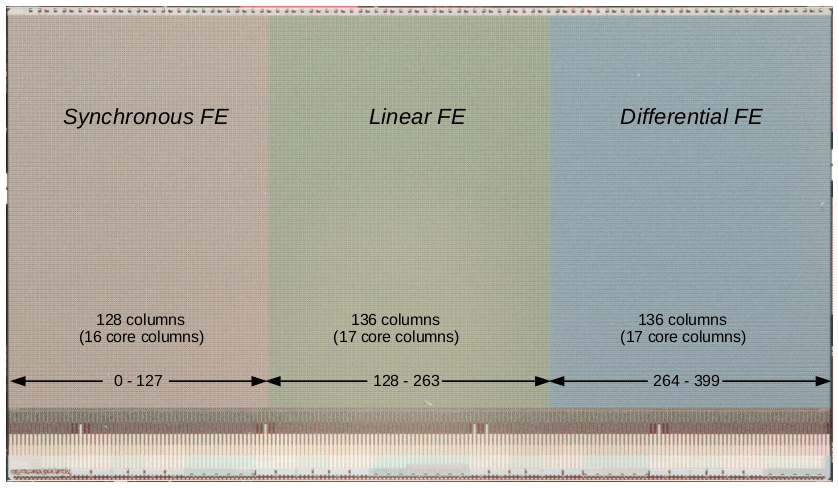
\includegraphics[scale=.3]{Immagini/FrontEnd}
\caption{Disposizione dei tre differenti \textit{front end} rispetto alla matrice di pixel.}
\label{FrontEnd}
\end{figure}

% Descriviamo ora brevemente il funzionamento di ciascuno dei tre Front End:

% \begin{itemize}

% \begin{figure}
% \centering
% 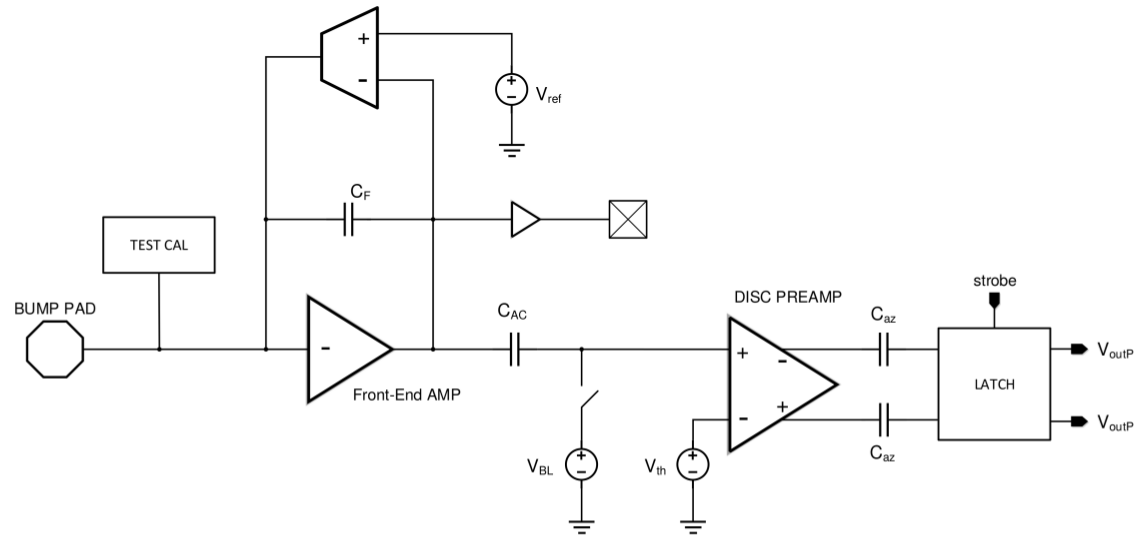
\includegraphics[width=\textwidth]{Immagini/SchemaSincrono}
% \caption{Schema semplificato del \textit{front end} Sincrono.}
% \label{SchemaSincrono}
% \end{figure}
% \item \textbf{Sincrono}. Il FE Sincrono, il cui schema è visibile in Fig.~\ref{SchemaSincrono}, \`e costituito da un amplificatore di carica (\textit{Charge Sensitive Amplifier} o CSA) a stadio singolo con un Krummenacher feedback accoppiato in AC ad un discriminatore sincrono, formato da un amplificatore differenziale e un latch di feedback positivo. 
% Il Krummenacher feedback è progettato in modo da compensare sia la corrente di buio del sensore sia la corrente di scarica della capacità presente nell'anello di reazione. 
% Maggiore la corrente maggiore la velocità con cui il segnale del preamplificatore torna al valore di \textit{baseline}.
% %Si tenga presente, come riferimento, che una carica di 10k$e^{-}$ e che produce un segnale di $10\nA$ di corrente e $400\ns$ di durata viene ridotta ad un segnale di $40\nA$ di corrente di $100\ns$.   
% %Per avere due differenti valori di guadagno, ci sono due capacità, rispettivamente di 2.5 fF e 4 fF. 
% A causa dei limiti della tecnologia a $65\nm$, si hanno fluttuazioni della \textit{baseline} in uscita dal primo stadio dell'ordine delle decine di millivolt tra un canale e l'altro e questa \`e la ragione dell'accoppiamento in AC del discriminatore. 
% In ogni caso le differenze tra transistor si traducono in un offset della tensione in uscita dal discriminatore tra i vari pixel. 
% Questo effetto, normalmente, è compensato con DAC locali che permettono regolazioni fini. 
% Nel FE Sincrono, invece, l'offset è compensato attraverso un meccanismo di auto azzeramento (\textit{auto zeroing}). 
% Per fare ciò è necessaria l'acquisizione del livello di tensione della \textit{baseline} ogni $100\us$s o meno.
% Durante le collisioni, la differenza tra segnale e baseline è inviata ad uno stadio di confronto che genera il segnale di uscita del discriminatore.

% \begin{figure}
% \centering
% 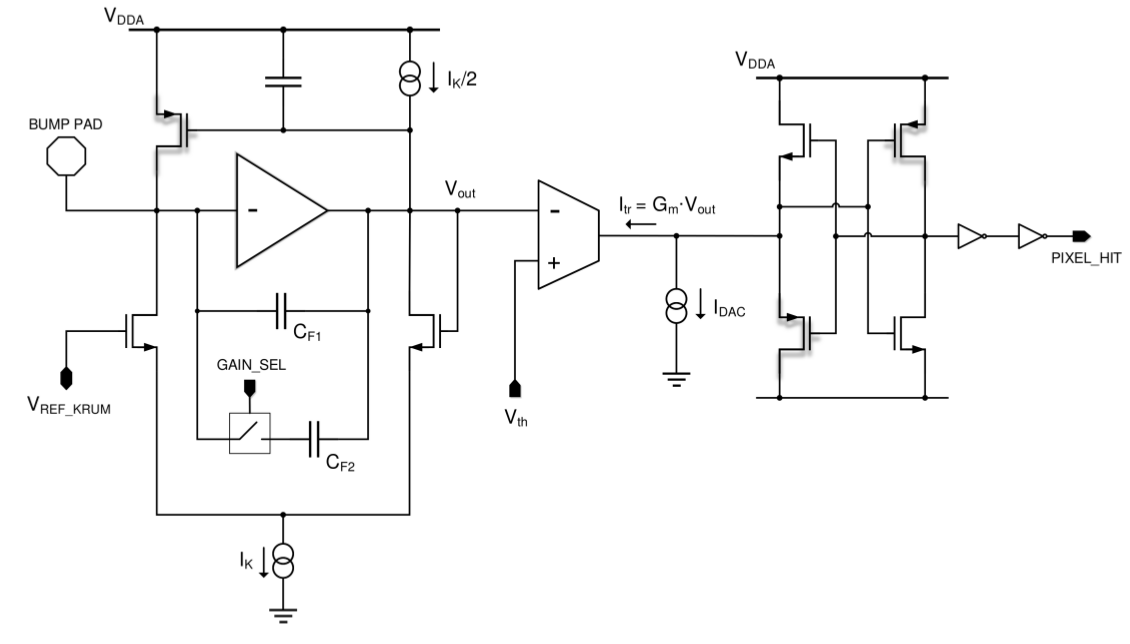
\includegraphics[width=\textwidth]{Immagini/SchemaLineare}
% \caption{Schema semplificato del \textit{front end} Lineare.}
% \label{SchemaLineare}
% \end{figure}
% \item \textbf{Lineare}. Lo schema semplificato del 
% Il FE Lineare è mostrato in Fig.~\ref{SchemaLineare}. Il circuito di lettura include un amplificatore di carica con un Krummenacher feedback per far fronte all'aumento di corrente di dispersione indotta dagli alti livelli di radiazione attesa. 
% La scelta di un amplificatore a stadio singolo è dettata dai limiti sui consumi e sullo spazio disponibile all'interno del chip. 
% Il segnale ottenuto dall'amplificatore di carica è mandato ad un comparatore che, insieme al contatore ToT (\textit{Time over Threshold}), è utilizzato per fare la conversione a segnale digitale. 
% Gli aggiustamenti della tensione di soglia sono gestiti, canale per canale, da un circuito locale basato su un \textit{binary weighted} DAC, a 4 bit, che genera una corrente $\mathrm{I_{DAC}}$, fornendo una regolazione locale della soglia. 
% Questo tipo di front end è stato ottimizzato per una carica massima di 30000 elettroni e un consumo complessivo di circa 4 $\mu$A. 
% L'amplificatore può essere utilizzato in regime di alto o basso guadagno, modificando il bit GAIN$\_$SEL, mentre la corrente di recupero, $\mathrm{I_K}$/2, proveniente dal circuito di Krummenacher feedback, può essere configurata tramite un DAC. 
% In configurazione di alto guadagno, per un segnale di carica pari a 30000, elettroni si ha un ToT di circa 400 ns, risultante in una corrente $\mathrm{I_K}$ di 25 nA. 
% La risoluzione attesa è di 15 mV/k$e^{-}$, mentre diventa di 7.5 mV/k$e^{-}$ in configurazione di basso guadagno. 
% Le prestazioni del preamplificatore di carica sono determinate, principalmente, dall'ingresso dell'amplificatore di carica e dalla parte del circuito di feedback con transistor PMOS. Dalle simulazioni il rumore in carica equivalente, per un rivelatore con capacità di 50 fF, è di 87 elettroni e, dopo la messa a punto, la dispersione della soglia scende da 380 a 35 elettroni.
% %Da simulazioni la dispersione della soglia dovrebbe passare da 380 elettroni a 35 elettroni dopo la messa a punto.

% \begin{figure}
% \centering
% 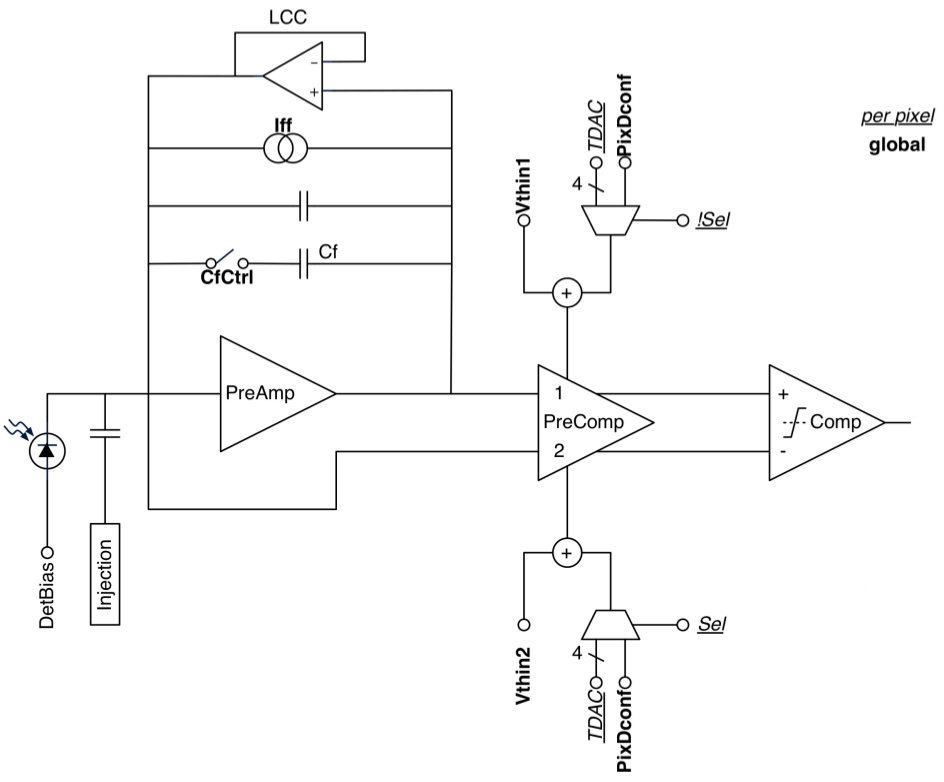
\includegraphics[scale=.3]{Immagini/SchemaDifferenziale}
% \caption{Schema semplificato del \textit{front end} Differenziale.}
% \label{SchemaDifferenziale}
% \end{figure}
% \item \textbf{Differenziale}. Il front end Differenziale è un circuito puramente analogico: non ha al suo interno latches, flip-flop o contatori. 
% I valori di configurazione sono, però, forniti da un nucleo digitale, che riceve dalla parte analogica solo il segnale in uscita del comparatore. 
% Naturalmente è necessaria la presenza di un ADC per la digitalizzazione del ToT ottenuto dal comparatore, anch'esso implementato interamente nella parte digitale. 
% Lo schema a blocchi del front end differenziale è riportato in figura \ref{SchemaDifferenziale}. 
% Il pre amplificatore, presente nel primo stadio, ha un guadagno continuo, regolabile tra i due valori di capacità presenti nell'anello di reazione.
% Il feedback in corrente è impostabile globalmente e non può essere regolato su ogni singolo pixel. 
% Dalle misure sui prototipi è stato visto che la dispersione nei valori di ToT che ne consegue ha un livello accettabile anche senza la necessità di una pre regolazione.  
% In caso di assenza di segnale, il feedback assicura che input e output del preamplificatore siano allo stesso potenziale.
% Nel secondo stadio, il pre comparatore fornisce un guadagno aggiuntivo e agisce come soglia differenziale.
% La soglia globale può essere regolata tramite le tensioni VTH1 e VTH2, mentre localmente la soglia è modificata utilizzando un \textit{resistor ladder} a 4 bit in ciascuno dei due rami del pre comparatore.
% Oltre ai 4 bit ce n'è un quinto che seleziona il ramo da modificare. 
% Dopo il pre comparatore si ha uno stadio con un comparatore, la cui uscita è collegata alla regione digitale tramite porte logiche. 
% Progettato per operare con una soglia di 500 elettroni, la parte analogica ha un consumo di 4$\mu$A/pixel, considerando una capacità di 50 fF e 10 nA di corrente dispersa.

% \end{itemize}

\section{Lo ShuntLDO di RD53A}
\begin{figure}
\centering
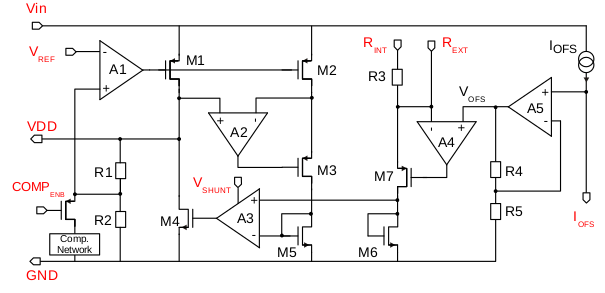
\includegraphics[width=\textwidth]{Immagini/SLDO_RD53A}
\caption{Regolatore LDO con Shunt (Shunt-LDO).}
\label{SLDO_RD53A}
\end{figure}
In RD53A l'alimentazione è gestita da due ShuntLDO, uno per la parte analogica ed uno per quella digitale, in cui la parte di potenza \`e distribuita nella periferia come descritto nella Sezione~\ref{Organizzazionechip}. Rispetto al circuito ShuntLDO prototipo a $2\A$ descritto nella Sezione~\ref{SLDO2A} presentato in precedenza, la tensione di offset $\mathrm{V_{ofs}}$ è generata con una circuiteria migliorata. Lo schema del circuito di ShuntLDO è riportato in Fig.~\ref{SLDO_RD53A}, mentre i pi\`u importanti parametri di funzionamento sono riportati in Tabella~\ref{tab:sldord53a}:

%\begin{center}
\begin{table}
\begin{small}
\noindent\setlength\tabcolsep{4pt}%
\begin{tabularx}{\linewidth}{|c|c|c|c|c|X|}
%\begin{tabular}{|c|c|c|c|c|l|}
\hline
\textbf{Pin} & \textbf{Tipologia} & \textbf{Min} & \textbf{Tipico} & \textbf{Max} & \textbf{Descrizione} \\ \hline
$\mathrm{V_{IN}}$ & Alimentazione & 1.4 V & & 2.0 V & Input di alimentazione esterna (in tensione)\\ \hline
 & Power & 0 A & 0.5 A & 2.0 A & Input di alimentazione esterna (in corrente)\\ \hline     
$\mathrm{V_{SHUNT}}$ & Alimentazione & 1.4 V & & 2.0 V & Tensione di alimentazione per il circuito di shunt\\ \hline
GND & Ground &  & &  & Terra locale e uscita della corrente di shunt\\ \hline
VDD & Alimentazione & 1.0 V & 1.2 V & 1.32 V & Tensione di uscita del regolatore\\ \hline
$\mathrm{V_{REF}}$ & Analogico & 500 mV & 600 mV & 660 mV & Tensione di riferimento (VDD=2$\mathrm{V_{REF}}$)\\ \hline
$\mathrm{R_{INT}}$ & Analogico &  & $\mathrm{V_{IN}}$ &  & Abilita la resistenza interna R\\ \hline
$\mathrm{R_{EXT}}$ & Analogico & 300 $\Omega$ &  &  & Resistenza esterna collegata a $\mathrm{V_{IN}}$\\ \hline
$\mathrm{I_{OFS}}$ & Analogico &  & 200 k$\Omega$ &  & Resistenza esterna connessa a GND\\ \hline
$\mathrm{COMP_{ENB}}$ & Digitale &  & GND &  & Segnale per abilitare il circuito di compensazione\\ \hline
\end{tabularx}
\end{small}
\caption{I pi\`u importanti parametri di funzionamento dello ShuntLDO di RD53A.}
\label{tab:sldord53a}
\end{table}
%\end{center}

Il valore di $\mathrm{V_{ofs}}$ è determinato tramite il terminale $\mathrm{I_{ofs}}$ previsto per connettervi un resistore $\mathrm{R_{iofs}}$ verso $GND$ definendo cos\`i la tensione $\mathrm{V_{+A5}}$ all'ingresso non invertente di A5. La sorgente di corrente $\mathrm{I_{ofs}}$ fornisce $2\uA$ e quindi
\begin{equation}
\label{eq:V+a5}
\mathrm{V_{+A5} = 2 \uA \cdot R_{iofs}}
\end{equation}
tensione che viene poi raddoppiata sull'ingresso di A4 tramite il partitore R4/R5 sull'anello di reazione di A5. Ne consegue che:
\begin{equation}
\label{eq:Vofs}
\mathrm{V_{ofs} = 2\cdot 2\uA \cdot R_{iofs}}.
\end{equation}
%\begin{equation}
%\mathrm{V_{in}= 2 \cdot V_{iofs} + \dfrac{R3}{1000} \cdot I_{in}}
%\end{equation}
Le misure presentate nelle sezioni successive sono stati ottenuti con i seguenti valori di R3 e $\mathrm{R_{iofs}}$:
\begin{center}
\begin{tabular}{lc}
\hline
$\mathrm{R3}$ & $600\Ohm$ \\%misurata con il multimetro è 620
$\mathrm{R_{iofs}}$ & $250\kOhm$\\ 
\hline
\end{tabular}
\end{center}
Tale valore di $\mathrm{R_{iofs}}$ corrisponde a $\mathrm{V_{+A5}\sim0.5\V}$ per cui, nell'andamento della tensione in ingresso in funzione della corrente ci aspettiamo un $\mathrm{V_{ofs}\sim 1\V}$.

Per quanto riguarda le tensioni di riferimento, come $\mathrm{V_{ref}}$, queste vengono generate all'interno del chip da un circuito bandgap dedicato.
La tensione di riferimento del bandgap è configurabile a passi di circa $1\mV$ tramite un registro a 5 bit il cui valore di default \`e 16, corrispondente a una tensione di circa $1.15\V$ che varia leggermente da un chip all'altro.
Un esempio è quello di figura \ref{bandgap_trimming}, in cui sono riportati, per differenti chip, gli andamenti misurati di $\mathrm{V_{ref}}$ al variare del valore impostato sul registro di configurazione. Per valori troppo piccoli di $\mathrm{V_{ref}}$ (che definiscono VDDA e VDDD) il ROC smette di funzionare e per questo motivo la parte sinistra del grafico non \`e popolata.
\begin{figure}
\centering
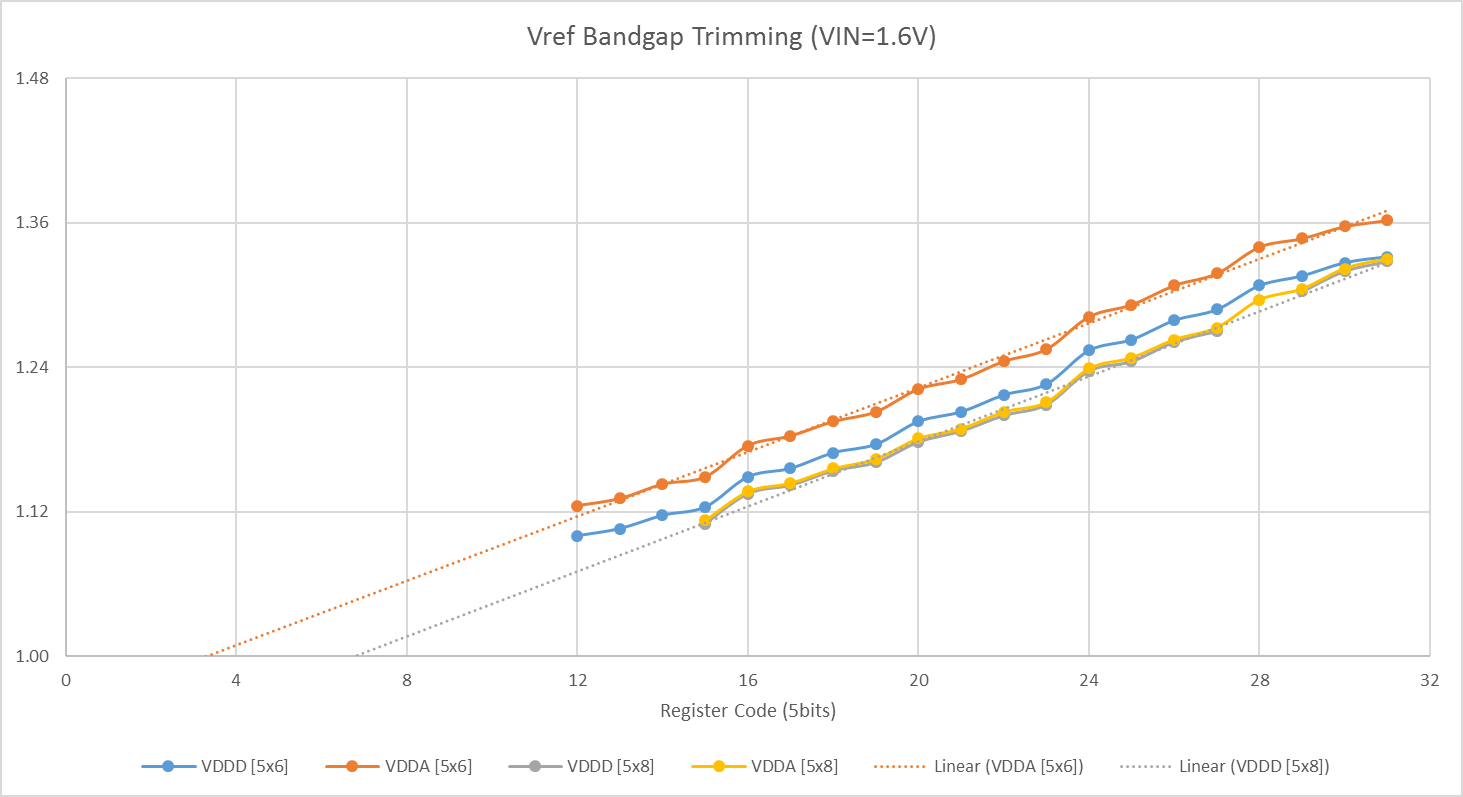
\includegraphics[scale=.5]{Immagini/bandgap_trimming}
\caption{Andamento della tensione $\mathrm{V_{ref}}$ generata internamente, per due diversi chip (per un totale di quattro bandgap), al variare del parametro di configurazione; il valore di default è 16. In due casi \`e riportata la retta di fit.}
\label{bandgap_trimming}
\end{figure}

\section{La Single Chip Card, scheda di test per RD53A}

Analogamente a quanto visto per gli ShuntLDO, che vengono collaudati usando una scheda di test, anche per il chip RD53A è necessaria una scheda di test detta \textit{Single Chip Card} (SCC) nella versione che ospita un solo ROC visibile in~Fig.~\ref{fig:RD53onSCC}.
\begin{figure}[t]
\centering
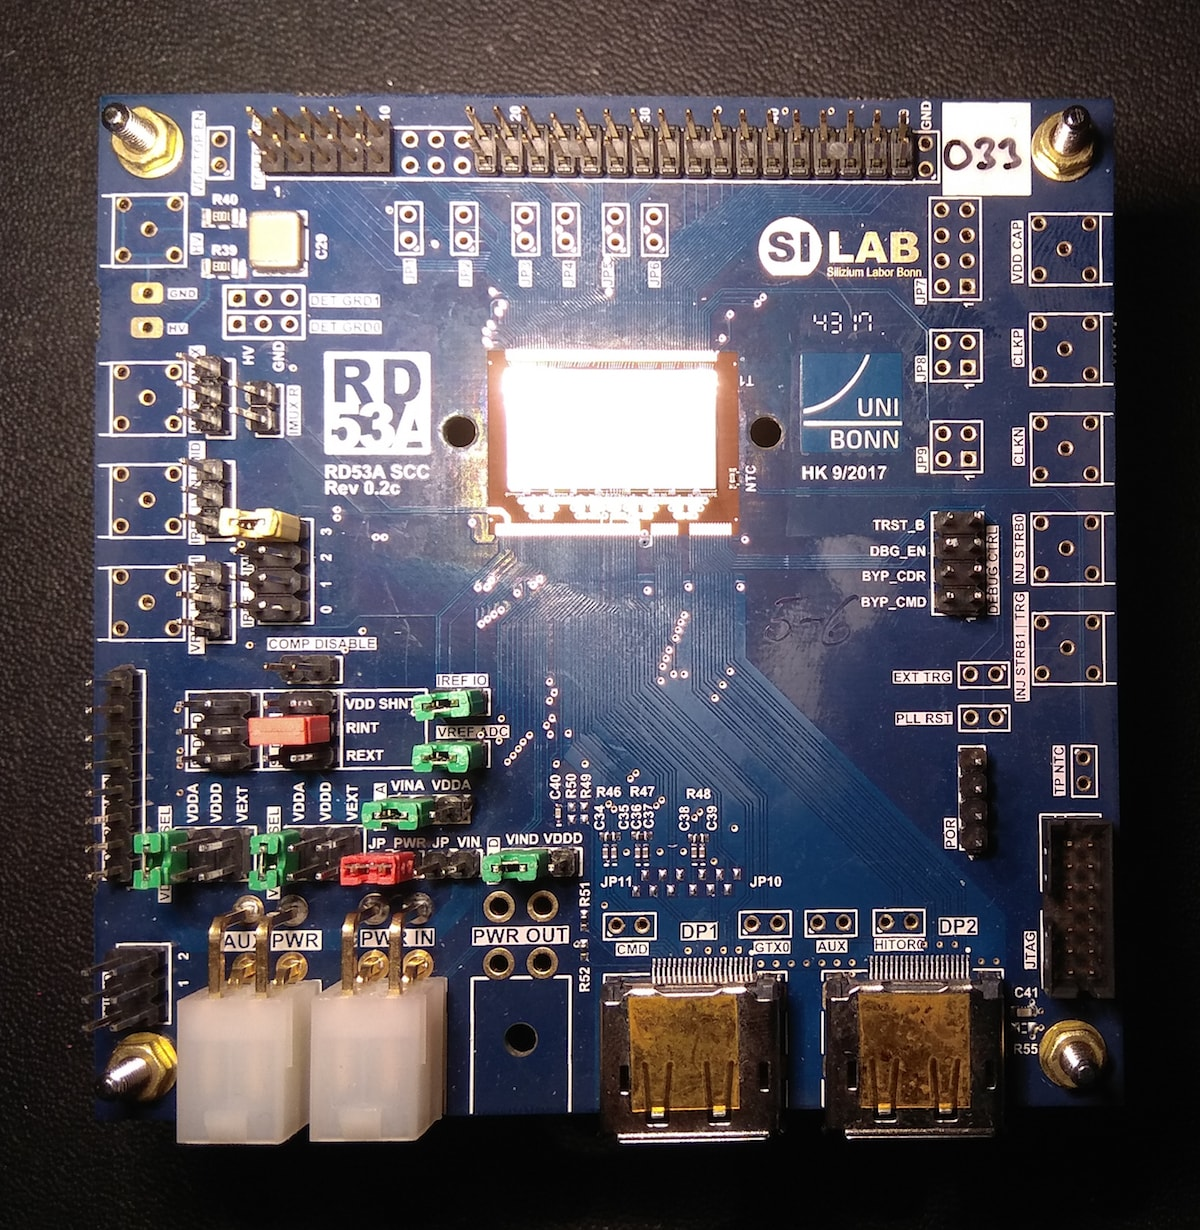
\includegraphics[width=0.4\textwidth]{Immagini/RD53onSCC.jpg}
\caption{Il prototipo di RD53A del gruppo di CMS di Firenze montato sulla sua SCC.}
\label{fig:RD53onSCC}
\end{figure}
 Il chip è fissato al centro di questa scheda e, attraverso microsaldature, è connesso ai vari elementi della scheda (terminali di monitoraggio, connettori di alimentazione, connettori con standard DisplayPort per la trasmissione/ricezione di dati, ponticelli/jumper di configurazione, ecc...). 
Il chip viene montato in un apposito spazio ai cui bordi arrivano le varie piste da connettere e sotto il quale un generoso strato metallico connesso tramite molti `via' al lato opposto della scheda assicura lo scambio termico consentendo, se necessario, l'applicazione di un sistema refrigerante o di un dissipatore sulla parte posteriore della SCC. 
Nel momento in cui l'alimentazione del chip viene fornita dai due ShuntLDO, infatti, la corrente non utilizzata viene dissipata sui due shunt che si scaldano rendendo quindi raccomandabile un minimo di raffreddamento per scongiurare la rottura del chip.
%La presenza di un raffreddamento è necessaria nel momento in cui l'alimentazione è data utilizzando i due ShuntLDO, infatti, la corrente non necessaria al chip viene dissipata sui due shunt che diventano punti molto caldi. 
%Al fine di evitare danneggiamenti del chip, e dell'eventuale sensore collegato, questo va raffreddato utilizzando dissipatori di calore. 

Dal momento che RD53A è un prototipo, si è lasciata la possibilità di configurare l'alimentazione esternamente, scegliendo tra tre diverse configurazioni.
Inoltre è possibile mantenere separate, a livello di alimentazione, la parte digitale e quella analogica quando, nel chip finale, si prevede che gli ShuntLDO della parte digitale e analogica saranno in parallelo. Le possibili configurazioni di alimentazione sono sotto elencate e in Fig.~\ref{SLDOmodes} sono riportati gli schemi di configurazione della SCC ad esse relativi.

\begin{description}
\item[Alimentazione con ShuntLDO] In questo caso il generatore utilizzato sarà in corrente. Per operare in configurazione ShuntLDO è necessario l'utilizzo di un sistema di raffreddamento per il chip che, in normali condizioni di lavoro, può essere un semplice dissipatore passivo. Nella misura delle varie tensioni, però, l'effetto di deriva termica non è trascurabile e, quindi, per le future misure, \`e in fase di preparazione un sistema di raffreddamento attivo che permetta di controllare le temperature.

\item[Alimentazione senza Shunt, con solo LDO] Questa configurazione necessita di una alimentazione in tensione e sarà il generatore esterno a dover fornire più o meno corrente in relazione ai consumi del chip. L'utilizzo del solo regolatore permette di avere un consumo ottimizzato in termini di potenza e, dunque, il chip pu\`o essere operato senza il bisogno di un sistema di raffreddamento.

\item[Alimentazione diretta] Lo ShuntLDO viene completamente escluso ed il chip è alimentato direttamente da un generatore di tensione esterno. L'alimentazione diretta deve essere utilizzata con particolare attenzione per evitare danneggiamenti del ROC. La presenza del regolatore LDO, infatti, anche privo di shunt, assicura che sbalzi di tensione all'ingresso dell'alimentazione non siano trasmessi al chip. Il regolatore, inoltre, tollera tensioni fino a 2 V, mentre il chip già sopra $\sim 1.3\V$ rischia di danneggiarsi. L'esclusione di questa sicurezza con la scelta di utilizzare un'alimentazione diretta è, perciò, sconsigliata. 
\end{description}

\begin{figure}[h]
\centering
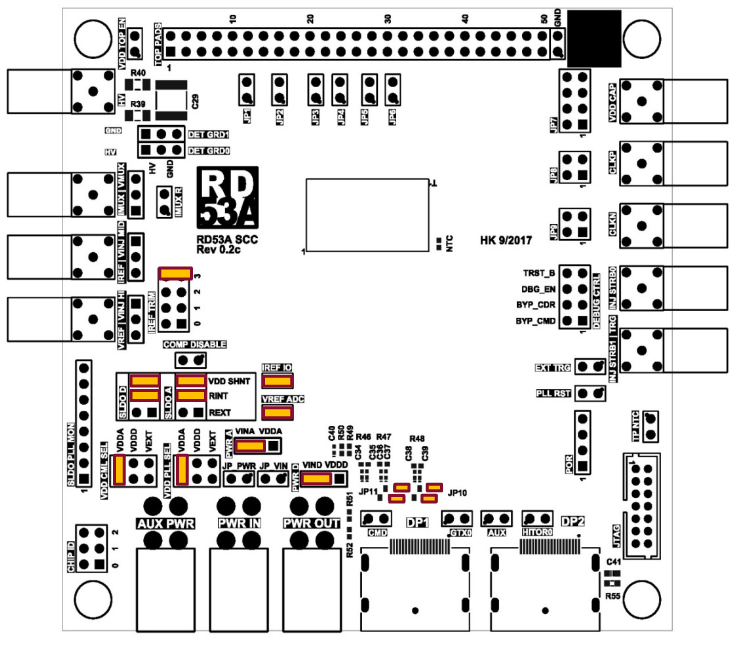
\includegraphics[width=0.25\textwidth]{Immagini/SLDOmode}
\hfill
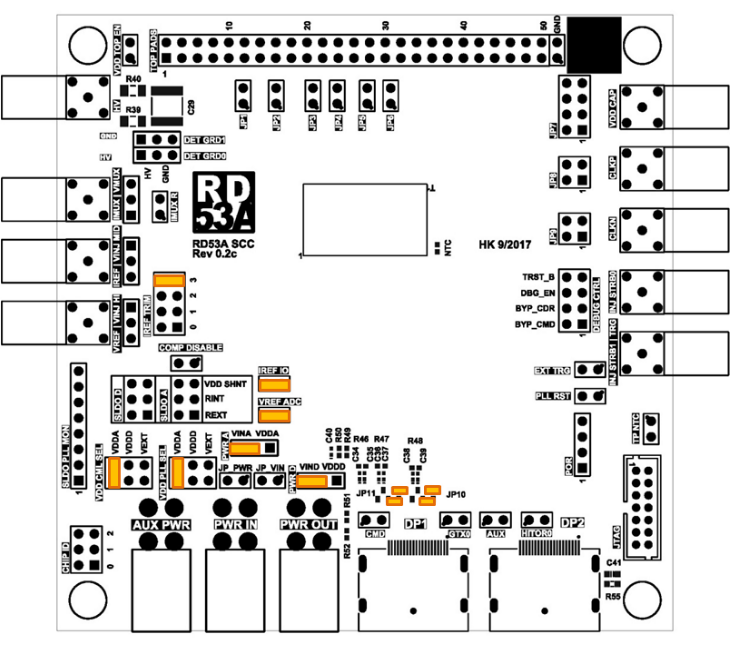
\includegraphics[width=0.25\textwidth]{Immagini/LDOmodeDefault}
\hfill
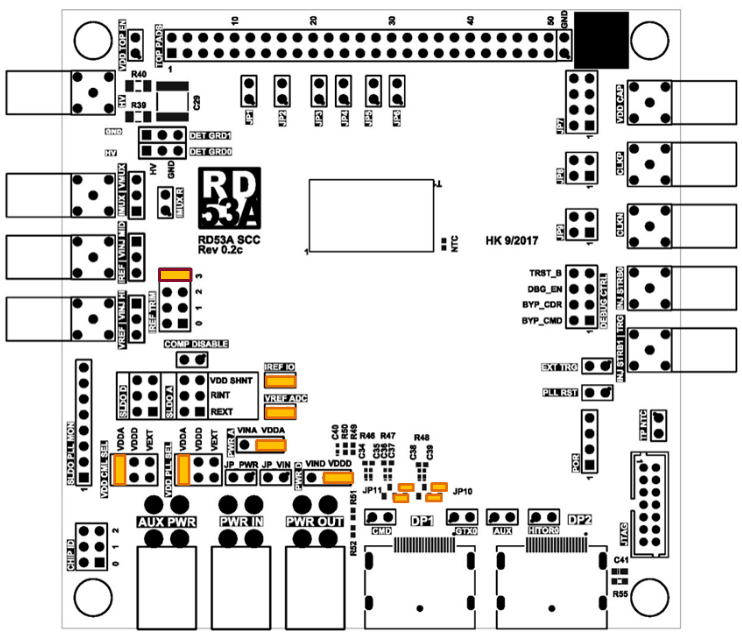
\includegraphics[width=0.25\textwidth]{Immagini/DirectPowering}
\caption{Disposizione dei jumper per le varie configurazioni di alimentazione dell'RD53A. Sinistra: ShuntLDO. Centro: LDO senza la parte di shunt. Destra: alimentazione diretta. In tutti e tre i casi la stessa configurazione \`e usata per la parte analogica e la parte digitale.}
\label{SLDOmodes}
\end{figure}

\section{Misure Statiche con RD53A}
\label{45}
Utilizzando il chip in configurazione ShuntLDO, raffreddato in modo passivo con un radiatore a contatto termico con il retro della SCC, si è proceduto alla caratterizzazione statica del comportamento dei due circuiti di alimentazione presenti nel chip rispettivamente per la parte analogica ed uno per quella digitale.

Questa studio è stato effettuato con diverse configurazioni risultanti dalla combinazione di tre aspetti operativi:
%Nel far questo sono state scelte diverse configurazioni, le scelte principali possono essere riassunte in tre punti:
\begin{itemize}
  \item alimentazione dei due regolatori con ShuntLDO: indipendenti o in parallelo fra loro;
  \item rampa di corrente crescente o decrescente;
  \item tensioni di riferimento $\mathrm{V_{ref}}$ e $\mathrm{V_{+A5}}$: generate internamente o fornite dall'esterno.
%\item Tenere i due regolatori con ShuntLDO in parallelo o con alimentazione indipendenti.
%\item Variare la corrente partendo da 0 A incrementandola via via o partendo da 1.5 A andando poi a decrescere.
%\item Utilizzare $\mathrm{V_{ref}}$ e $\mathrm{V_{iofs}}$ generati internamente o fornirli esternamente.
\end{itemize}

In tabella~\ref{tab:legenda} è riportata la descrizione delle abbreviazioni utilizzate per le legende dei grafici.
\begin{table}
\begin{center}
%\noindent\setlength\tabcolsep{4pt}%
\begin{tabular}{c|l}
%\begin{tabularx}{\linewidth}{c|r}
%\multicolumn{2}{|c|}{Abbreviazione} & \multicolumn{1}{c|}{\multirow{2}{*}{Descrizione}}\\ 
 Abbreviazione & Descrizione\\ \hline
\multicolumn{2}{l}{Parte Analogica} \\
\hline
VINA & Tensione $\mathrm{V_{INA}}$ all'ingresso del regolatore  \\ \hline
VDDA & Tensione $\mathrm{V_{outA}}$ all'uscita del regolatore \\ \hline
$\mathrm{V_{iofs \_ m \_ A}}$ & $\mathrm{V_{+A5A}}$ \\ \hline   
$\mathrm{V_{ref \_ m \_ A}}$  & $\mathrm{V_{refA}}$ \\ \hline \hline  
\multicolumn{2}{l}{Parte Digitale} \\ \hline
% Abbreviazione & Descrizione\\ 
VIND & Tensione $\mathrm{V_{IND}}$ all'ingresso del regolatore  \\ \hline
VDDD & Tensione $\mathrm{V_{outD}}$ all'uscita del regolatore \\ \hline
$\mathrm{V_{iofs \_ m \_ D}}$ & $\mathrm{V_{+A5D}}$ \\ \hline   
$\mathrm{V_{ref \_ m \_ D}}$  & $\mathrm{V_{refD}}$ \\ 
\end{tabular}
\end{center}
\caption{Descrizione delle abbreviazioni utilizzate per le legende dei grafici.}
\label{tab:legenda}
\end{table}

\subsubsection{Alimentazioni indipendenti, rampa di corrente crescente, tensioni di riferimento interne}
\label{sec:iui}

\begin{figure}
\centering
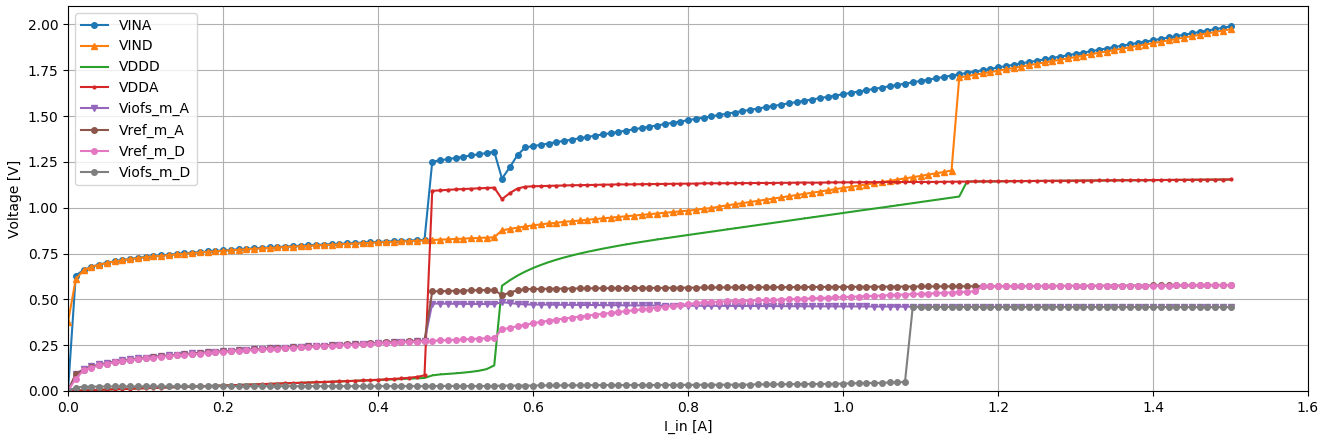
\includegraphics[width=\textwidth]{Immagini/IUI2}
\caption{Grafici tensione-corrente ottenuti tenendo i due regolatori separati e variando le rispettive correnti $\mathrm{I_{in}}$ da $0\A$ a $1.5\A$.}%allungare descrivendo anche l'undershoot
\label{IUI}
\end{figure}
Le prime misure sono state eseguite utilizzando, come riferimento per $\mathrm{V_{out}}$ e $\mathrm{V_{iofs}}$, le tensioni generate internamente al chip.
La corrente fornita ai due ShuntLDO, alimentati indipendentemente, è stata variata, contemporaneamente, da $0\A$ a $1.5\A$ a passi di $10\mA$.
L'andamento ottenuto è quello riportato in Fig.~\ref{IUI}.

La fluttuazione verso il basso ben visibile sulle tensioni della parte analogica, sia in ingresso che in uscita, è causata da uno sbilanciamento nella distribuzione delle correnti nei due ShuntLDO: quando si attiva la parte digitale si ha un picco di assorbimento di corrente a scapito della parte analogica che risulta nelle fluttuazioni riassunte in tabella.
\begin{center}
\begin{tabular}{ccc}
\hline
$\Delta \mathrm{V_{INA}}$ & $\Delta \mathrm{V_{refA}}$ &$\Delta \mathrm{V_{outA}}$  \\ \hline
$\sim$0.150 V & $\sim$ 0.030 V& $\sim$0.060 V\\ \hline     
\end{tabular}.
\end{center}
Questo fenomeno è stato osservato nonostante la configurazione sia tale da avere i due ShuntLDO, per la parte digitale e analogica, alimentati separatamente, segno che, all'interno del chip, sono presenti fenomeni di `dialogo' fra i due ambiti: un po' di corrente scorre attraverso le connessioni tra le due regioni, causando la caduta di tensione osservate nella parte analogica.
%Questo avviene nonostante le alimentazioni dei due ShuntLDO siano separate, in quanto all'interno del chip ci sono zone di 'dialogo' tra regione analogica e digitale. 
%Si ha scorrimento di corrente attraverso connessioni tra le due regioni che causano cadute di tensioni nella parte analogica, questo comportamento è pericoloso e va evitato. 
Questo comportamento è potenzialmente dannoso perch\'e pu\`o alterare la corretta sequenza di accensione con il rischio di fenomeni di oscillazione o che il ROC finisca in uno stato anomalo senza possibilit\`a di recupero.

Inoltre, sempre dalla Fig.~\ref{IUI}, si può notare che VDDD sale parzialmente quando $\mathrm{I_{in}}$ raggiunge $\sim0.56\A$, non riuscendo però ad andare a regime, poiché la tensione $\mathrm{V_{IND}}$ non è ancora sufficientemente abbastanza elevata da consentire una corretta regolazione. Questo, a sua volta, è dovuto al ritardo con cui $\mathrm{V_{+A5D}}$ raggiunge il valore corretto, solo per $\mathrm{I_{in}\sim 1.1\V}$. Infatti, come introdotto in precedenza, la tensione  $\mathrm{V_{+A5D}}$ è ottenuta dalla caduta di tensione sulla resistenza $\mathrm{R_{iofs}}$, nel nostro caso di $\sim 250\kOhm$, indotta dalla corrente $\mathrm{I_{ofs} \sim 2 \uA}$. Se, per vari motivi, il circuito che genera questa corrente ha un ritardo nell'accensione, questo si ripercuote nell'accensione del ROC nel suo complesso.  

Questa discussione illustra come le problematiche di {\em power-on} siano cruciali e crescano di complessit\`a quando il circuito base (lo ShuntLDO nel nostro caso) viene vestito con tutta la circuiteria addizionale. Il ROC finale per l'IT dovr\`a essere progettato per essere completamente affidabile rispetto al {\em power on} che, tradizionalmente, \`e un aspetto delicato dell'elettronica digitale. Questo \`e vero in particolare in presenza del danneggiamento da radiazione che altera le caratteristiche circuitali per cui, potenzialmente, certe problematiche possono non essere presenti nel ROC non irraggiato e comparire dopo che lo stesso ha integrato una certa fluenza. La validazione del ROC non pu\`o prescidere da una estesa campagna di test dopo irraggiamento.

Le cause del diverso comportamento di $\mathrm{V_{+A5A}}$ e $\mathrm{V_{+A5D}}$ rispetto ai valori di corrente $\mathrm{I_{in}}$ che sono necessari perch\`e queste due tensioni raggiungano il livello nominale non sono comprese al momento. Da disegno i due ShuntLDO e i relativi circuiti addizionali per la parte analogica e la parte digitale sono gemelli e quindi questa differenza \`e inaspettata e probabilmente dovuta a effetti spuri di power-on. Infatti questa asimmetria scompare effettuando la misura una rampa di corrente inversa come illustrato nella prossima sezione.

%\begin{center}
%\begin{tabular}{|l|c|c|c|c|}
%\hline
% & \multicolumn{2}{c|}{Digitale} & \multicolumn{2}{c|}{Analogica} \\ \hline
% 
%& media & errore & media & errore \\ \hline
%
%$\mathrm{R_{eq}}$ & 0.752 $\Omega$ & 0.0003 $\Omega$& 0.7178 $\Omega$ & 0.0003 $\Omega$ \\ \hline
%$\mathrm{V_{ofs}}$ & 0.844 V& 0.004 V & 0.9025 V & 0.0003 V\\ \hline     
%
%\end{tabular}
%\end{center}

%\begin{figure}
%\centering
%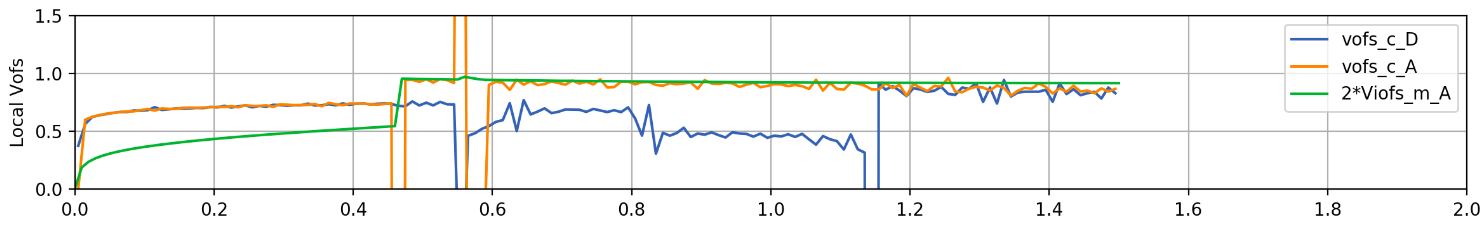
\includegraphics[scale=.27]{Immagini/IUISubPlotVofs}
%\caption{.}
%\label{IUISubPlotVofs}
%\end{figure}

%\begin{center}
%\begin{tabular}{|l|c|c|}
%\hline
%&Digitale  &Analogica \\ \hline
%$\mathrm{R_{eq}}$ & 0.753 $\Omega$& 0.724 $\Omega$ \\ \hline
%$\mathrm{V_{ofs}}$ & 0.845 V & 0.900 V\\ \hline
%\end{tabular}
%\end{center}

\subsubsection{Alimentazioni indipendenti, rampa di corrente decrescente, tensioni di riferimento interne}

\begin{figure}
\centering
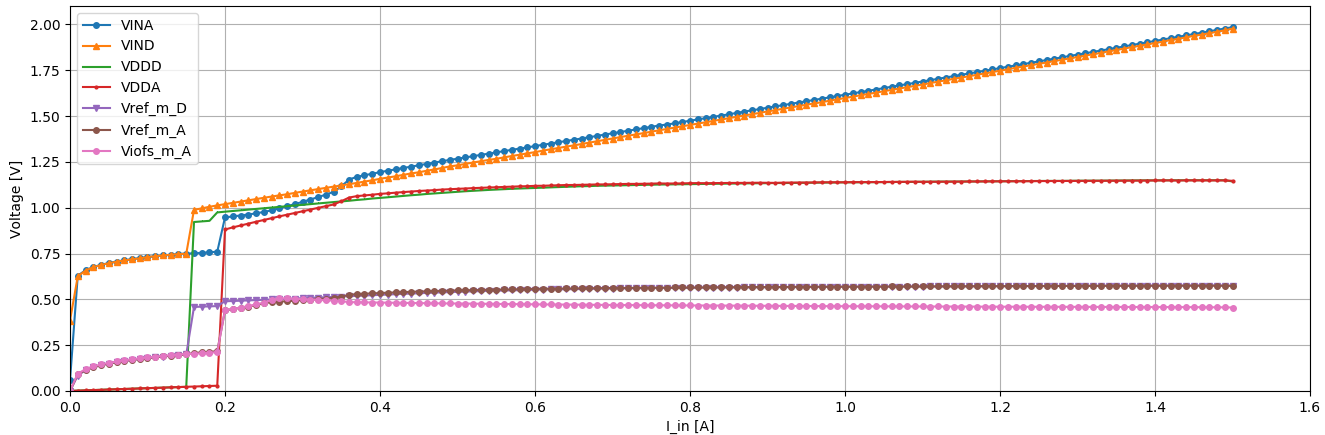
\includegraphics[width=\textwidth]{Immagini/IDI2}
\caption{Grafici tensione-corrente ottenuti tenendo i due regolatori separati e variando le rispettive correnti $\mathrm{I_{in}}$ da $1.5\A$ a $0\A$.}
\label{IDI}
\end{figure}

Per verificare che i comportamenti anomali descritti nella sezione precendente siano effettivamente legati alla sequenza interna di accensione, si sono ripetute le misure effettuando la scansione in corrente in senso inverso partendo da $\mathrm{I_{in}}\sim1.5\A$ per poi scendere fino a $0\A$. Dagli andamenti mostrati in Fig.~\ref{IDI}, si può notare come siano scomparse le fluttuazioni presenti nella precedente scansione, in accordo con l'ipotesi che queste siano dovute alla parziale attivazione del ROC che risulta compiuta solo per valori pi\`u elevati di $\mathrm{I_{in}}$. 

In assenza di un segnale di clock esterno, il ROC, nella configurazione di default, richiede circa $50\mA$ per la parte digitale e $400\mA$ per quella analogica.
%Questo fin tanto che il chip non riceve un segnale di clock esterno. 
Questa differenza in consumi di corrente si riflette nel fatto che, diminuendo la corrente, il comparto analogico \`e il primo a mostrare problemi con un primo flesso poco i sotto $400\mA$ circa e spegnendosi a $200\mA$ circa. La parte digitale, invece, rimane attiva anche con correnti inferiori.

Partendo da valori di corrente elevati, inoltre, e quindi da tensioni in ingresso ben al di sopra di quelle strettamente necessarie, non si osservano neppure i problemi dovuti ai differenti istanti di accensione delle parti analogica e digitale.
%\begin{center}
%\begin{tabular}{|l|c|c|c|c|}
%\hline
% & \multicolumn{2}{c|}{Digitale} & \multicolumn{2}{c|}{Analogica} \\ \hline
% 
%& media & errore & media & errore \\ \hline
%
%$\mathrm{R_{eq}}$ & 0.73475 $\Omega$ & 0.00008 $\Omega$& 0.7153 $\Omega$ & 0.0006 $\Omega$ \\ \hline
%$\mathrm{V_{ofs}}$ & 0.86530 V& 0.00007 V & 0.9043 V & 0.0005 V\\ \hline     
%
%\end{tabular}
%\end{center}

\subsubsection{Alimentazioni indipendenti, rampa di corrente crescente, $\mathrm{V_{ref}}$ esterna} 

\begin{figure}
\centering
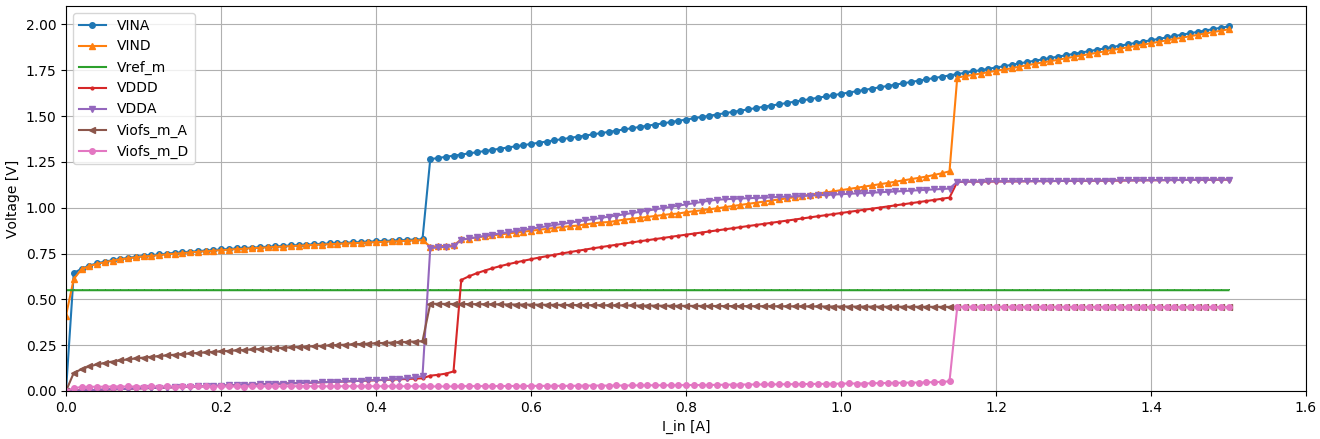
\includegraphics[width=\textwidth]{Immagini/IUEVref2}
\caption{Grafici tensione-corrente ottenuto tenendo i due regolatori separati e variando le rispettive correnti $\mathrm{I_{in}}$ da $0\A$ a $1.5\A$, utilizzando un riferimento esterno $\mathrm{V_{ref}}=0.550 \V$ sia per la parte analogica che digitale.}
\label{IUEVref}
\end{figure}
Continuando a tenere i due circuiti di alimentazione separati è interessante studiare, per confronto, il comportamento nel caso in cui le tensioni di riferimento non siano generate dal ROC stesso.
I grafici riportati in Fig.~\ref{IUEVref} sono ottenuti fornendo esternamente $\mathrm{V_{ref}}=0.550\V$,  sia per la parte analogica che per quella digitale.
Il comportamento della parte digitale è analogo a quello ottenuto di cui in Fig.~\ref{IUI}, mentre, per la parte analogica, non si hanno le fluttuazione osservate n\'e su $\mathrm{V_{INA}}$ n\'e $\mathrm{V_{outA}}$. $\mathrm{V_{outA}}$, però, risente ancora del comportamento della parte digitale: fino a che $\mathrm{V_{ofsD}}$ non arriva al valore nominale per tramite di $\mathrm{V_{+A5D}}$, $\mathrm{V_{outA}}$ non si stabilizza.

%\begin{center}
%\begin{tabular}{|l|c|c|c|c|}
%\hline
% & \multicolumn{2}{c|}{Digitale} & \multicolumn{2}{c|}{Analogica} \\ \hline
% 
%& media & errore & media & errore \\ \hline
%
%$\mathrm{R_{eq}}$ & 0.7539 $\Omega$ & 0.00007 $\Omega$& 0.7448 $\Omega$ & 0.0002 $\Omega$ \\ \hline
%$\mathrm{V_{ofs}}$ & 0.84199 V& 0.00011 V & 0.8706 V & 0.0003 V\\ \hline     
%
%\end{tabular}
%\end{center}

%
% ---------------------- Sono arrivato qui
%

\subsubsection{Alimentazioni indipendenti, rampa di corrente crescente, $\mathrm{V_{+A5}}$ esterna} 

\begin{figure}
\centering
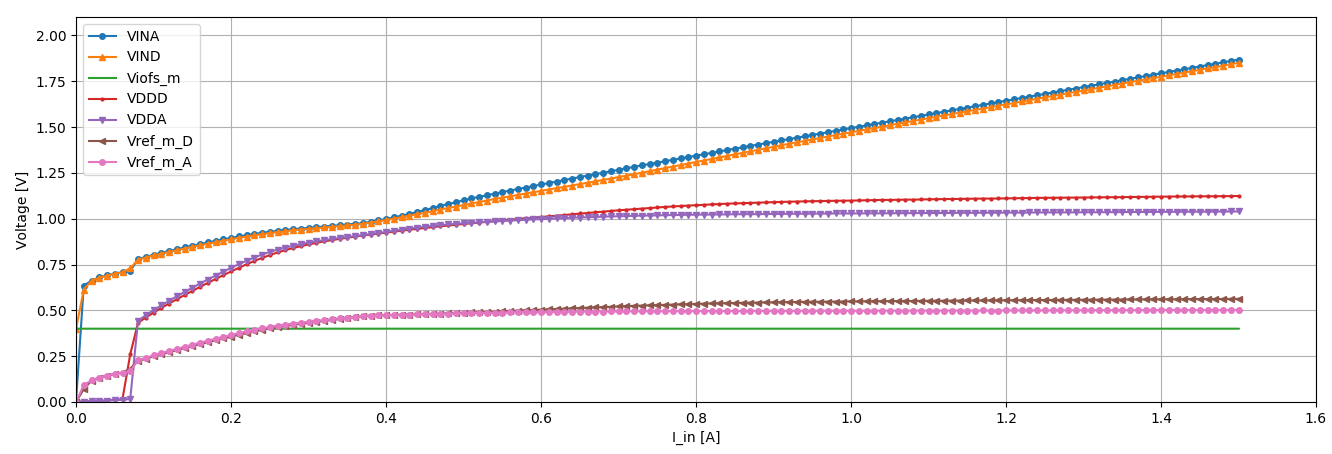
\includegraphics[width=\textwidth]{Immagini/IUEViofs2}
\caption{Grafici tensione-corrente ottenuto tenendo i due regolatori separati e variando le rispettive correnti $\mathrm{I_{in}}$ da $0\A$ a $1.5\A$, utilizzando un riferimento esterno $\mathrm{V_{+A5}}=0.400\V$ sia per la parte analogica che digitale.}
\label{IUEViofs}
\end{figure}
 Le stesse misure sono state ripetute fornendo esternamente il solo $\mathrm{V_{+A5}}=0.400 \V$ e utilizzando $\mathrm{V_{ref}}$ interno sia per la parte analogica che digitale e tenendo le alimentazioni dei due ShuntLDO indipendenti. In questo caso gli andamenti ottenuti sono decisamente migliori, come si vede in Fig.~\ref{IUEViofs}. 
Infatti, i $\mathrm{V_{+A5}}$ esterni permettono di evitare le problematiche precedentemente riscontrate quali i differenti valori di corrente $\mathrm{I_{in}}$, tra parte analogica e digitale, oltre i quali si entra in regime di regolazione. Questo grazie al fatto che il valore di $\mathrm{V_{ofs}}$, grazie al pilotaggio esterno, \`e fissato al valore nominale. %\begin{center}
%\begin{tabular}{|l|c|c|c|c|}
%\hline
% & \multicolumn{2}{c|}{Digitale} & \multicolumn{2}{c|}{Analogica} \\ \hline
% 
%& media & errore & media & errore \\ \hline
%
%$\mathrm{R_{eq}}$ & 0.7871 $\Omega$ & 0.0013 $\Omega$& 0.7554 $\Omega$ & 0.0013 $\Omega$ \\ \hline
%$\mathrm{V_{ofs}}$ & 0.6824 V& 0.0013 V & 0.7403 V & 0.0012 V\\ \hline     
%
%\end{tabular}
%\end{center}

%\begin{figure}
%\centering
%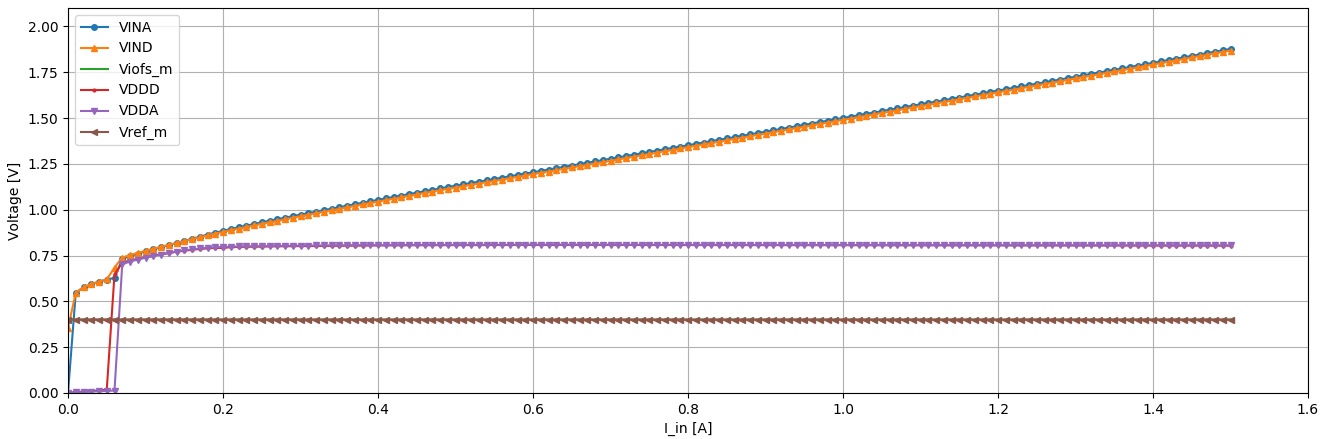
\includegraphics[scale=.3]{Immagini/IUEAll}
%\caption{IUEAll viofs e vref si sovrappongono .}
%\label{IUEAll}
%\end{figure} 
%Infine riportiamo il grafico degli andamenti nal caso in cui sia $\mathrm{V_{ref}}$ che $\mathrm{V_{iofset}}$ sono forniti esternamente. entrambi valgono 0.400, mancanza di kitley

%\begin{center}
%\begin{tabular}{|l|c|c|c|c|}
%\hline
% & \multicolumn{2}{c|}{Digitale} & \multicolumn{2}{c|}{Analogica} \\ \hline
% 
%& media & errore & media & errore \\ \hline
%
%$\mathrm{R_{eq}}$ & 0.7461 $\Omega$ & 0.0004 $\Omega$& 0.7448 $\Omega$ & 0.0004 $\Omega$ \\ \hline
%$\mathrm{V_{ofs}}$ & 0.7452 V& 0.0004 V & 0.7563 V & 0.0004 V\\ \hline 
%\end{tabular}
%\end{center}  

\subsubsection{Alimentazione in parallelo, rampa di corrente crescente, tensioni di riferimento interne} 

\begin{figure}[h]
\centering
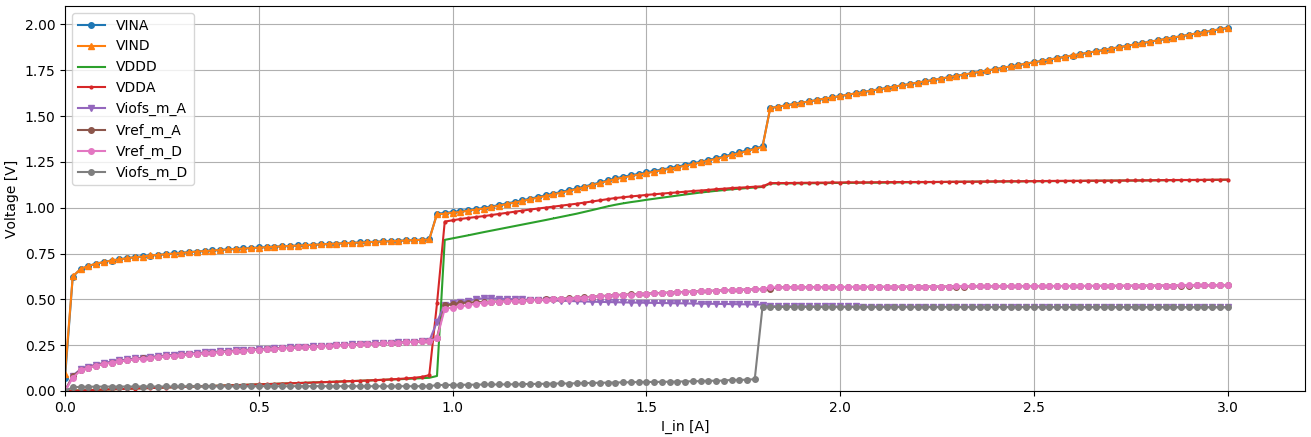
\includegraphics[width=\textwidth]{Immagini/PUI}
\caption{Grafici tensione-corrente ottenuti con i due regolatori in parallelo e variando la corrente totale, riportata sull'asse delle ascisse, da $0\A$ a $3\A$.}
\label{PUI}
\end{figure}
Come detto in precedenza, in RD53A è stata lasciata la possibilità di tenere separate le alimentazioni dei due ShuntLDO, mentre nella versione finale i due ShuntLDO si troveranno in parallelo. 
In questa configurazione gli andamenti delle tensioni in ingresso ($\mathrm{V_{INA}}$ e $\mathrm{V_{IND}}$) e di quelle in uscita ($\mathrm{V_{outA}}$ e $\mathrm{V_{outD}}$) risultano migliori, nonostante che $\mathrm{V_{ofsA}}$ e $\mathrm{V_{ofsD}}$ raggiungano il valore nominale per differenti valori di $\mathrm{I_{inA}}$ e $\mathrm{I_{inD}}$ , rispettivamente, come si può vedere in Fig.~\ref{PUI}.
Questo miglioramento nel comportamento può essere attribuito all'utilizzo dell'alimentazione in parallelo dei due ShuntLDO, poiché la corrente totale a disposizione si può suddividere in modo ottimale tra i due ambiti, come effettivamente accade. Questo sbilanciamento nella ripartizione delle correnti si verifica nell'intervallo di correnti in cui $\mathrm{V_{+A5A}}$ \`e gi\`a al valore nominale mentre $\mathrm{V_{+A5D}}$ non lo \`e ancora, come risulta evidente se confrontiamo la Fig.~\ref{CurrentSharing} con gli andamenti di $\mathrm{V_{+A5A}}$ e $\mathrm{V_{+A5D}}$ nella~Fig.~\ref{PUI}.

%\begin{center}
%\begin{tabular}{|l|c|c|c|c|}
%\hline
% & \multicolumn{2}{c|}{Digitale} & \multicolumn{2}{c|}{Analogica} \\ \hline
% 
%& media & errore & media & errore \\ \hline
%
%$\mathrm{R_{eq}}$ & 0.7441 $\Omega$ & 0.0002 $\Omega$& 0.7396 $\Omega$ & 0.0009 $\Omega$ \\ \hline
%$\mathrm{V_{ofs}}$ & 0.8635 V& 0.003 V & 0.8688 V & 0.0011 V\\ \hline 
%\end{tabular}
%\end{center}

\begin{figure}
\centering
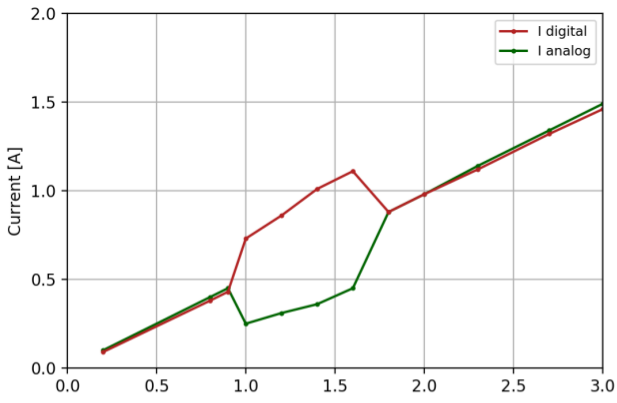
\includegraphics[scale=.4]{Immagini/CurrentSharing}
\caption{Misura della suddivisione della corrente tra i due regolatori posti in parallelo; in ascissa è riportata la corrente totale fornita al parallelo.}%meeting del 16 aprile
\label{CurrentSharing}
\end{figure}
Il comportamento descritto è simile a quanto riportato in letteratura~\cite{SLDO} nel caso in cui, per\`o, i due ShuntLDO siano configurati per fornire due tensioni $\mathrm{V_{outA}}$ e $\mathrm{V_{outB}}$ diverse. In particolare si osserva uno sbilanciamento di corrente quando solo uno degli ShuntLDO \`e in regime di regolazione. Sbilanciamento che scompare quando la fase di accensione \`e completata per entrambi.
 
%, la distribuzione delle correnti torna ad essere bilanciata. 
%Questo comportamento è noto e compreso: il meccanismo che lo innesca risiede nell'offset dell'amplificatore A2, utilizzato nel \textit{current mirror}. 
%L'offset, infatti, implica un differente $\mathrm{V_{DS}}$ tra i transistor M1 e M2 influenzando il rapporto k nella regione lineare.
%Dunque, fintantoché in uno dei due regolatori la tensione di uscita è minore di quella di riferimento, si ha uno sbilaciamento delle correnti. 
%Quando viene raggiunto il livello di riferimento, M1 e M2 saturano e l'effetto dell'offset svanisce.
%Questo problema, che si verifica durante l'accensione, può essere mitigato utilizzando particolari architetture con basso offset per l'amplificatore A2.

\subsubsection{Confronti fra le varie configurazioni}

Da ciascuna delle configurazioni discusse nei paragrafi precedenti sono stati ricavati, per la regione di regolazione, i parametri fondamentali $\mathrm{V_{ofs}}$ e $\mathrm{R_{eff}}$ della curva caratteristica $\mathrm{V_{IN}}$ vs. $\mathrm{I_{IN}}$. Idealmente ci aspettiamo che la pendenza sia confrontabile con $\sim\nicefrac{\mathrm{R3}}/1000$ e $\mathrm{V_{ofs}}$ con il doppio di $2\times \mathrm{V_{+A5}}$. A questo proposito ricordiamo che i valori nominali sono 
\begin{center}
\begin{tabular}{lc}
\hline
$\mathrm{R3}$ & $600\kOhm$ \\%misurata con il multimetro è 620
$\mathrm{V_{+A5}}$ & $0.5\V$\\
\hline
\end{tabular}
\end{center}

In tabella~\ref{table:results} sono riportati i risultati di questa analisi. Riguardo alla descrizione della configurazione è specificato se i due regolatori sono alimentati in parallelo o indipendentemente, se la corrente è stata fatta variare in modo crescente o decrescente e se le tensioni di riferimento $\mathrm{V_{+A5}}$, $\mathrm{V_{refA}}$ e $\mathrm{V_{refB}}$ sono generate internamente o esternamente al ROC.
\begin{center}
\begin{table}
\begin{tabular}{l|c|c|c|c|c|c|c|c}
Regolatore & Alim. & Rampa & \multicolumn{2}{c|}{$\mathrm{V_{ref}}$} & \multicolumn{2}{c|}{$\mathrm{V_{+A5}}$} & $\mathrm{R_{eff}}$& $\mathrm{V_{ofs}}$ \\
Regolatore & Alim. & Rampa & \multicolumn{2}{c|}{[V]}               & \multicolumn{2}{c|}{[V]}                & [$\Omega$]       & [V]               \\ \hline
Analogico & \multirow{2}{*}{Indip.} & \multirow{2}{*}{Cres.} & Int. & - & Int. & - & 0.72 & 0.90 \\
Digitale  &  &  & Int. & - & Int. & - & 0.75  & 0.84 \\ \hline

Analogico & \multirow{2}{*}{Indip.} & \multirow{2}{*}{Decr.} & Int. & - & Int. & - & 0.71 & 0.90 \\
Digitale  &  &  & Int. & - & Int. & - & 0.73  & 0.86 \\ \hline

Analogico & \multirow{2}{*}{Indip.} & \multirow{2}{*}{Cres.} & Ext. & 0.550 & Int. & - & 0.75 & 0.87 \\
Digitale  &  &  & Ext. & 0.550 & Int. & - & 0.75  & 0.84 \\ \hline

Analogico & \multirow{2}{*}{Indip.} & \multirow{2}{*}{Cres.} & Int. & - & Ext. & 0.400 & 0.75 & 0.74 \\
Digitale  &  &  & Int. & - & Ext. & 0.400 & 0.79  & 0.68 \\ \hline

Analogico & \multirow{2}{*}{Paral.} & \multirow{2}{*}{Cres.} & Int. & - & Int. & - & 0.74 & 0.87 \\
Digitale  &  &  & Int. & - & Int. & - & 0.74  & 0.86 \\
\end{tabular}
\caption{Valori di $\mathrm{V_{ofs}}$ e $\mathrm{R_{eff}}$ ricavati da un fit alla caratteristica $\mathrm{V_{IN}}$ vs. $\mathrm{I_{IN}}$ nella regione di regolazione dei i due ShuntLDO a seconda della configurazione.}
\label{table:results}
\end{table}
\end{center}

I risultati sono stati ottenuti mediando pi\`u caratteristiche tensione-corrente effettuate nella stessa configurazione. I valori di tensione misurati per una data $\mathrm{V_{IN}}$ sono molto stabili all'interno di ciascun gruppo (variazioni assolute inferiori a $3\mV$, tipicamente di $\sim 1\mV$), mentre i valori estratti di $\mathrm{R_{eff}}$ e di $\mathrm{V_{ofs}}$ variano fra una configurazione e l'altra.
%La prima cosa che si può notare è che i valori variano da una configurazione all'altra, mentre mantenendo per una stessa configurazione rimangono pressochè uguali, infatti i risultati sono stati ottenuti mediando su più misure.
Gli errori statistici associati alla stima di $\mathrm{R_{eff}}$ e di $\mathrm{V_{ofs}}$ sono trascurabili rispetto alle fluttuazioni di questi parametri nelle diverse configurazioni e rispetto ad altri possibili contributi sistematici alle incertezze coem, ad esempio, le variazioni di temperatura. 

\begin{figure}
\centering
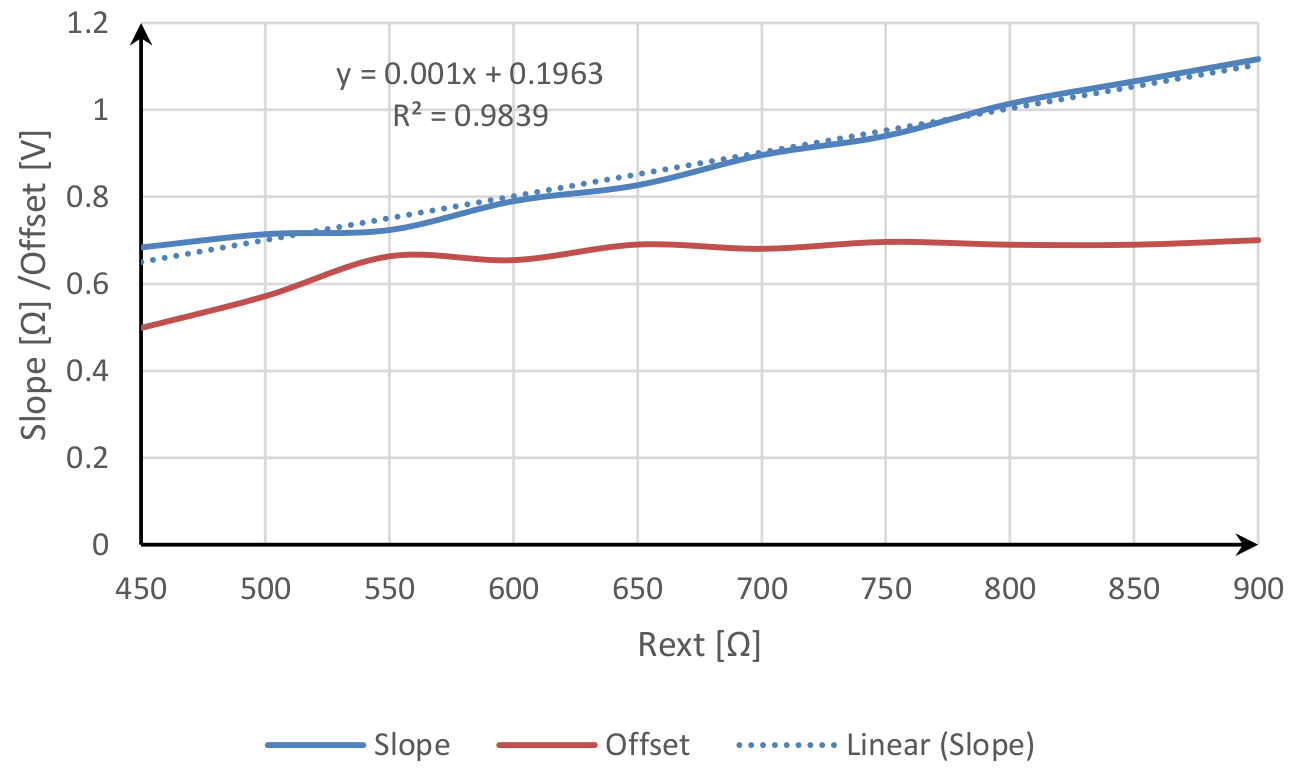
\includegraphics[width=\textwidth]{Immagini/R3Karagounis}
\caption{Andamento di $\mathrm{R_{eff}}$ e $\mathrm{V_{ofs}}$ al variare della resistenza esterna $\mathrm{R_{ext}}$ utilizzata per definire la corrente nel ramo di controllo dello ShuntLDO.}%meeting del 13 aprile R^2 https://en.m.wikipedia.org/wiki/Coefficient_of_determination
\label{R3Karagounis}
\end{figure}
Dal confronto con i valori attesi risulta evidente che la pendenza della caretteristica tensione-corrente nella regione di regolazione degli ShuntLDO misurati è sistematicamente maggiore mentre l'offset è sistematicamente minore. 
Questo comportamento è stato osservato in tutti gli esemplari di RD53A utilizzati per lo sudio degli ShuntLDO. \`E stata eseguita, in particolare, una misura dedicata a queste discrepanze studiando l'andamento di $\mathrm{R_{eff}}$ e $\mathrm{V_{ofs}}$ al variare della resistenza $\mathrm{R3}$, ottenuto grazie ad un resistore esterno $\mathrm{R_{ext}}$ regolabile e riportato in Fig.~\ref{R3Karagounis}. La relazione che ne risulta, $\mathrm{R_{eff}} = 0.001\cdot \mathrm{R_{ext}} + 0.1963\Ohm$, si discosta da quella di progetto $\mathrm{R_{eff} = \nicefrac{R_{ext}}{k} = \nicefrac{R3}{k}}$ (con $k=1000$) per la presenza del termine costante pari a circa $0.2\Ohm$ dovuto a qualche contributo spurio che probabilmente varia da esemplare a esemplare. Questa misura conferma i risultati precedentemente ottenuti e giustifica la sistematica osservazione di una $\mathrm{R_{eff}}$ pi\`u grande di quella aspettata. 

Per quanto riguarda l'osservazione di valori di $\mathrm{V_{ofs}}$ inferiori a quanto atteso il fenomeno è di più difficile interpretazione.
%In parte è dovuto alla differenza tra terra del chip e terra dello shunt?!.
\begin{figure}
\centering
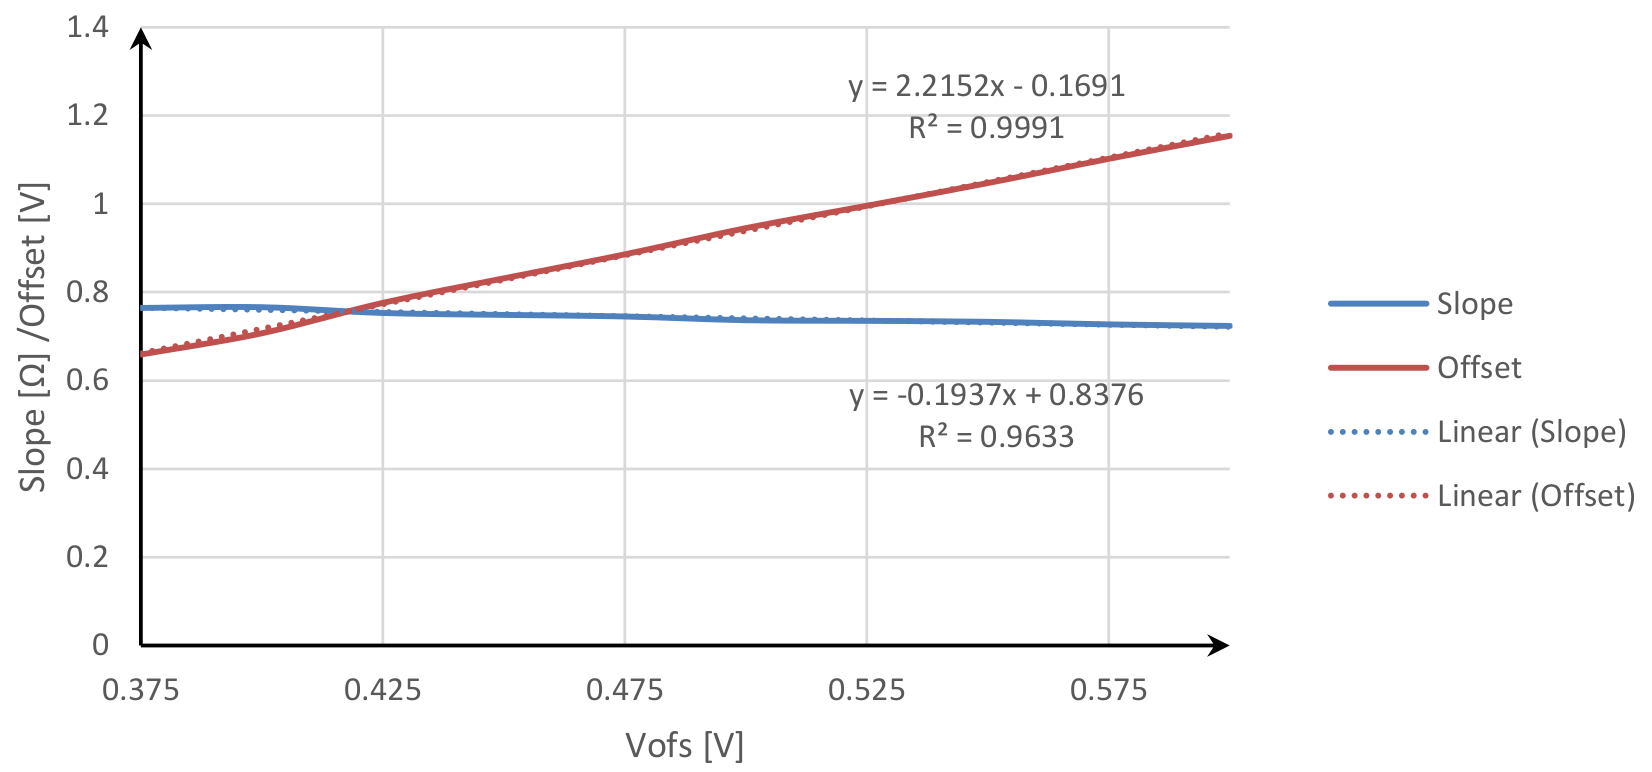
\includegraphics[width=\textwidth]{Immagini/OffsetKaragounis}
\caption{Andamento di $\mathrm{R_{eff}}$ e $\mathrm{V_{ofs}}$ al variare della tensione $\mathrm{V_{+A5}}$ fornita esternamente.}%meeting del 13 aprile
\label{OffsetKaragounis}
\end{figure}
In questo caso l'andamento di $\mathrm{R_{eff}}$ e $\mathrm{V_{ofs}}$ al variare della tensione $\mathrm{V_{+A5}}$ fornita esternamente visibile in Fig.~\ref{OffsetKaragounis}, mostra che $\mathrm{V_{ofs} = 2.215\cdot V_{+A5}- 0.169\V}$. Il fattore moltiplicativo \`e maggiore di circa il 10\% rispetto a quello di progetto nominalmente pari a 2. Inoltre \`e presente un termine costante non nullo. Infine, entrambe le misure delle Figure~\ref{R3Karagounis} e ~\ref{OffsetKaragounis} suggeriscono l'esistenza di una correlazione tra $\mathrm{V_{ofs}}$ e $\mathrm{R_{eff}}$. L'origine di questi comportamenti anomali rispetto al progetto del ROC non \`e nota al momento ma studi approfonditi e simulazioni sono in corso per per comprenderne le cause ed eliminarle.

%
% ------------------------------------
%
\subsection{Variazioni di carico}
\label{451}
\begin{figure}
\centering
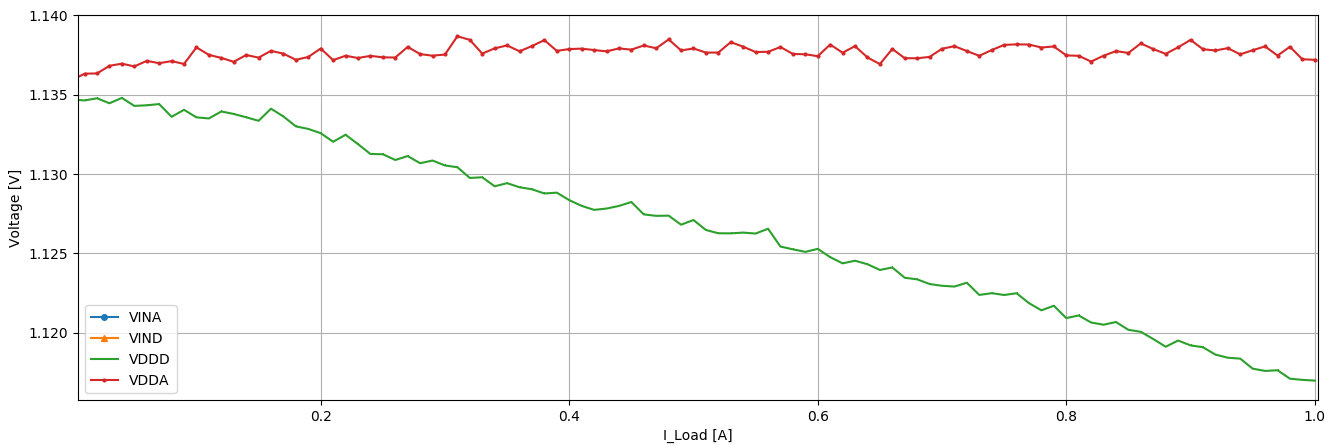
\includegraphics[width=\textwidth]{Immagini/LoadVDDD}
\caption{Andamento della tensione di alimentazione della parte analogica VDDA e digitale VDDD in funzione della corrente assorbita in più dal carico applicato allo ShuntLDO digitale.}
\label{LoadVDDD}
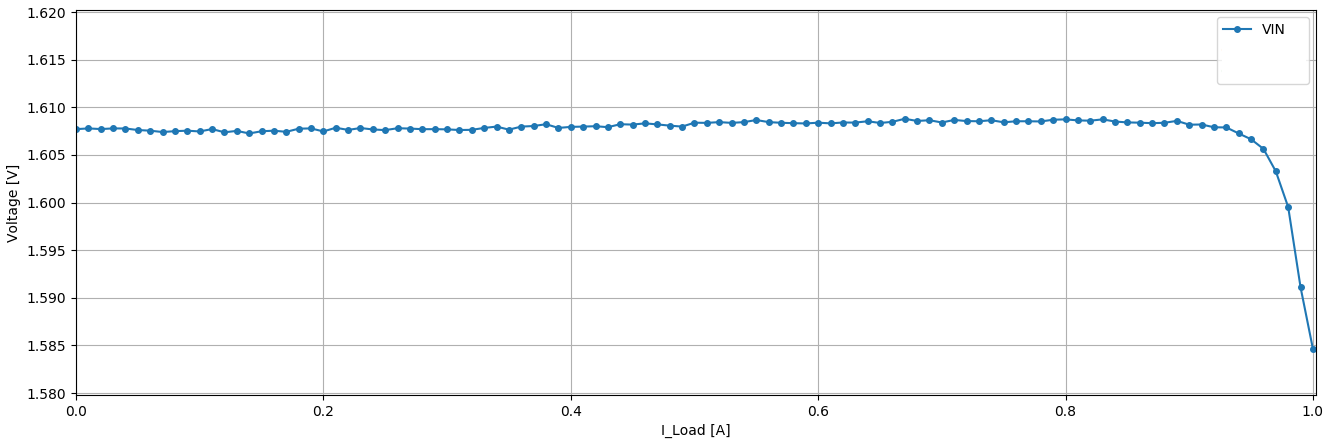
\includegraphics[width=\textwidth]{Immagini/LoadVIND}
\caption{Andamento della tensione di ingresso del chip in funzione della corrente assorbita in più dal carico applicato allo ShuntLDO digitale.}
\label{LoadVIND}
\end{figure}

Per lo ShuntLDO il carico è rappresentato dal chip, che fino a che si trova nella configurazione di default, ha consumi di corrente tipici pari a:
\begin{center}
\begin{tabular}{cc}
\hline
Regione Analogica & Regione Digitale \\ \hline
$\sim$0.400 A & $\sim$ 0.050 A\\ \hline     
\end{tabular}
\end{center}
Le misure riportate di seguito sono ottenute al variare del carico che applicato al VDDD/VDDA, ponendo in parallelo al chip un alimentatore Keithley utilizzato come sink di corrente. 
Come configurazione del chip si è utilizzato lo ShuntLDO con i due circuiti di alimentazione in parallelo. 
La corrente in ingresso è stata fissata a 2 A, corrispondenti ad 1 A per ciascun ShuntLDO. 
Dati i diversi consumi tra parte analogica e digitale, l'intervallo di variazione del carico è stato scelto diversamente per le due: tra 0 A e 1 Aper la parte digitale, tra 0 A e 0.69 A per l'analogica. 
Queste variazioni di carico non sono dinamiche, ma vanno considerate come statiche, infatti le tensioni di ingresso e di uscita vengono misurate, ad ogni incremento del valore del carico, su tempi scala lunghi rispetto a quelli di risposta del circuito di ShuntLDO. 
Gli andamenti riportati di seguito vanno, quindi, interpretati come una deriva del valore della tensione prodotta dal regolatore in funzione dell'entità del carico. 
In figura \ref{LoadVDDD} sono mostrati gli andamenti ottenuti con il carico applicato alla parte digitale.
Come si può vedere, la tensione di alimentazione della regione digitale diminuisce gradualmente, arrivando ad una variazione di $\sim$18 mV per un carico addizionale di 1 A.
La parte analogica, invece, non risente di queste variazioni e rimane costante. %pendenza 18 mOhm(ogni 100 mA 1.8 mV
L'andamento della tensione in ingresso, figura \ref{LoadVIND}, ha invece una caduta di $\sim$24 mV che però si concentra nella parte finale partendo per valori di carico di circa 0.940 A.
Questo comportamento è plausibile se si considera che, da sola, la parte digitale consuma 50 mA e, dunque, la somma delle correnti assorbite tra chip e carico supera  quella a disposizione di 1 A. 
\begin{figure}
\centering
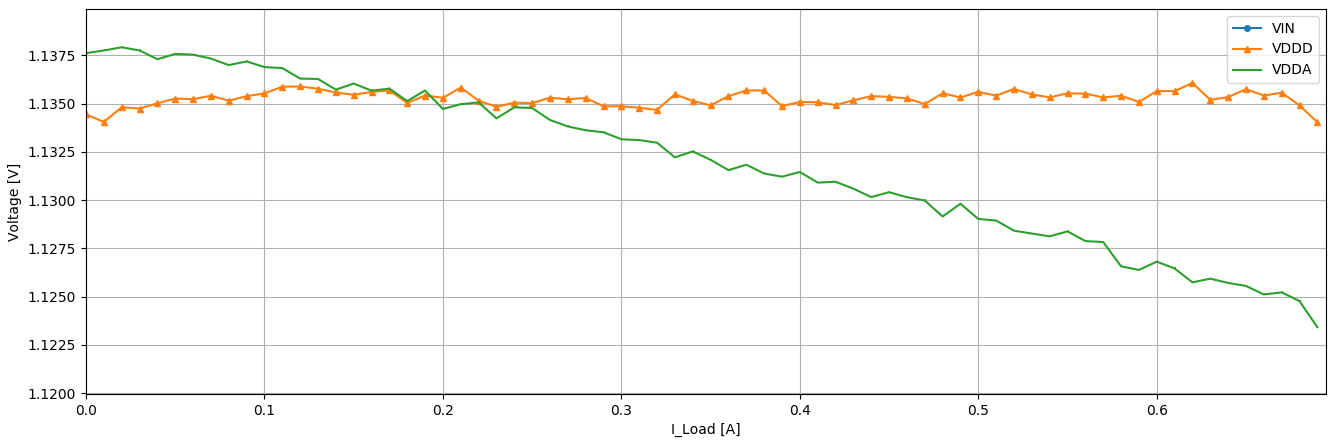
\includegraphics[width=\textwidth]{Immagini/LoadVDDA}
\caption{Andamento della tensione di alimentazione della parte analogica VDDA e digitale VDDD in funzione della corrente assorbita in più dal carico applicato allo ShuntLDO analogico.}
\label{LoadVDDA}
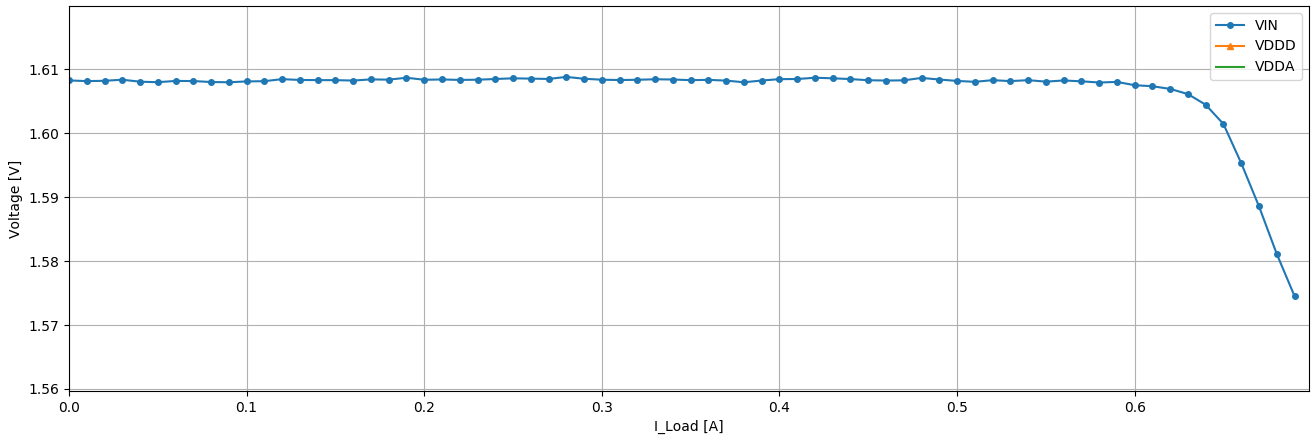
\includegraphics[width=\textwidth]{Immagini/LoadVINA}
\caption{Andamento della tensione di ingresso del chip in funzione della corrente assorbita in più dal carico applicato allo ShuntLDO analogico.}
\label{LoadVINA}
\end{figure}
Un discorso analogo si può fare per la parte analogica, tenendo presente che i consumi minimi per il chip sono $\sim$400 mA.
L'andamento della tensione prodotta dal regolatore è riportata in figura \ref{LoadVDDA}, mentre, per quanto riguarda quella in ingresso il grafico di riferimento è quello di figura \ref{LoadVINA}. 
Per la tensione di uscita la caduta è di $\sim$15 mV per un carico di 0.690 A, %21mOhm
per quella in ingresso si ha, invece, una diminuzione di $\sim$26 mV in corrispondenza di un carico di 0.690 A, anche in questo caso il consumo totale di corrente supera 1 A. 
La diminuzione di tensione per $\mathrm{V_{in}}$ inizia con un carico di $\sim$0.610 A.


Un'altra misura di interesse è quella relativa alle fluttuazioni della tensione generata dallo ShuntLDO per variazioni repentine del carico, in funzione del margine di corrente fornito Fig.~\ref{LoadTransient}. 
Questi risultati sono stati ottenuti andando ad abilitare e disabilitare il clock su parte dei canali di lettura, questo causa una variazione della corrente assorbita dalla sola parte digitale, che quindi è soggetta a fluttuazioni di tensione più o meno importanti.

\begin{figure}
\centering
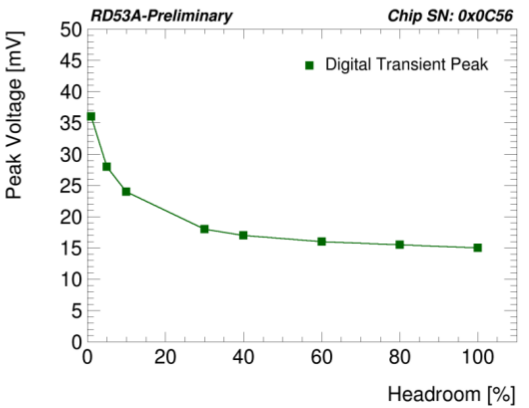
\includegraphics[width=0.65\textwidth]{Immagini/LoadTransientDominik}
\caption{Il grafico riporta il valore di picco della variazione della tensione VDDD  in funzione del margine di corrente dato su 1 A di alimentazione nel caso in cui  i consumi di parte analogica e digitale sono entrambi $\sim$0.5 A, la fluttuazione è ottenuta abilitando e disabilitando il segnale di clock per una parte dei canali di lettura. 100$\%$ significa che la corrente fornita al chip è 1 A+1 A.}
\label{LoadTransient}
\end{figure}

\subsection{Fast ramp-up}

\begin{figure}
\centering
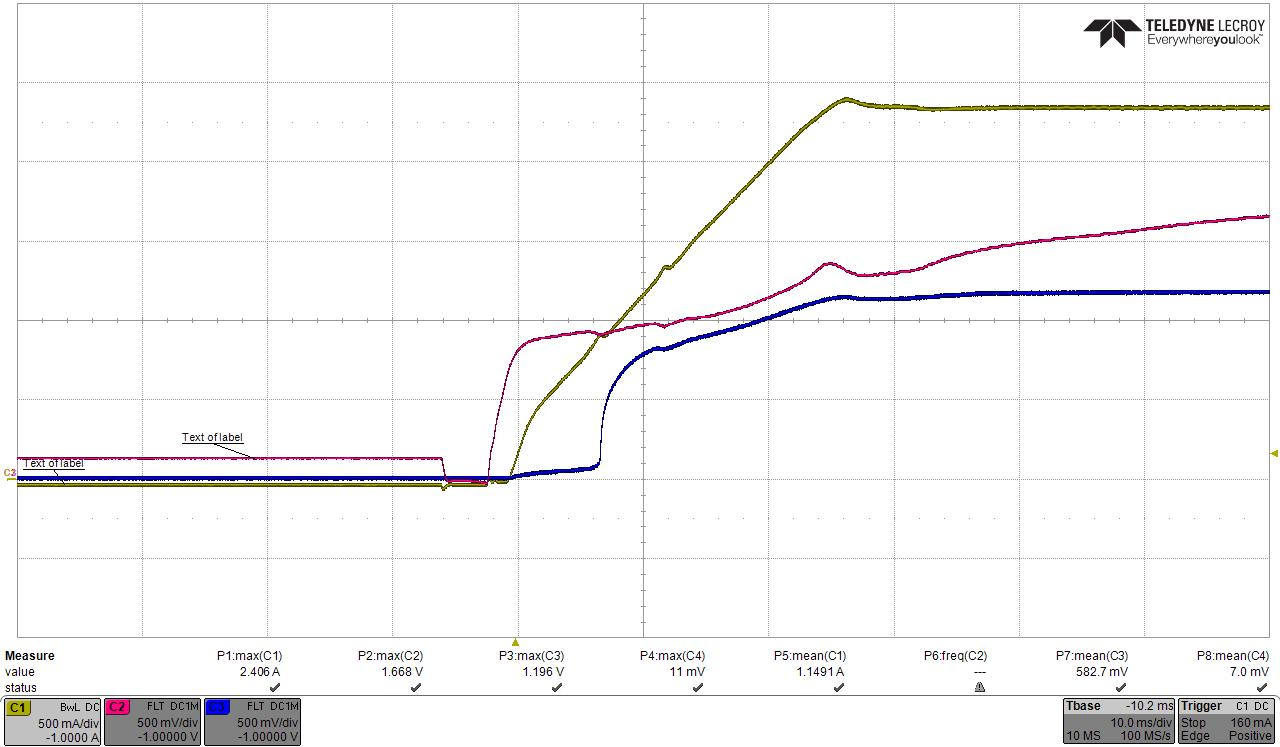
\includegraphics[scale=.3]{Immagini/rd-powup-dir6}
\caption{In giallo è riportata la corrente che in 25 ns passa da 0 A a 2.4 A, in fucsia la tensione in ingresso e in blu la tensione con cui è alimentata la parte digitale del chip VDDA.}
\label{rd-powup-dir6}
\end{figure}

\begin{figure}
\centering
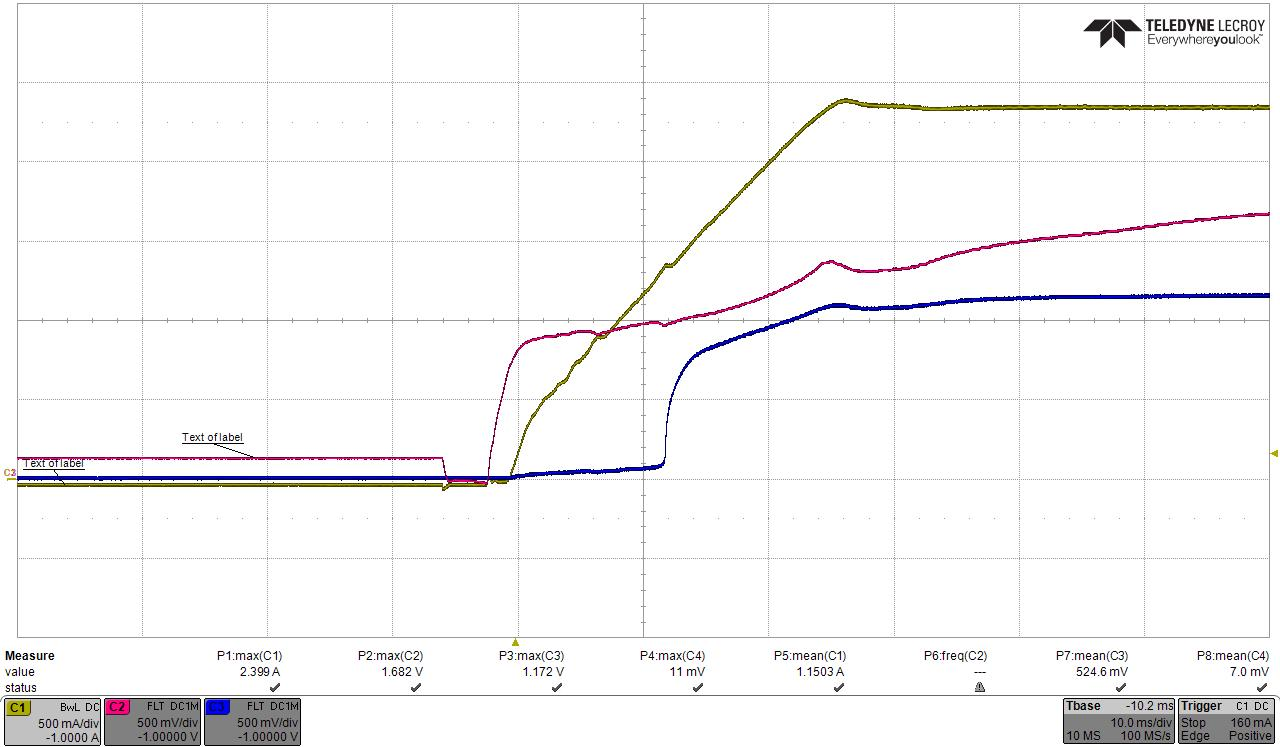
\includegraphics[scale=.3]{Immagini/rd-powup-dir7}
\caption{In giallo è riportata la corrente che in 25 ns passa da 0 A a 2.4 A, in fucsia la tensione in ingresso e in blu la tensione con cui è alimentata la parte analogica del chip VDDD.}
\label{rd-powup-dir7}
\end{figure}

Le misure riportate fino ad ora, sullo studio dei circuiti di ShuntLDO in RD53A, sono da considerarsi statiche, in quanto sono ottenute su tempi scala lunghi in confronto a quello di risposta dello ShuntLDO. 
%Fino ad ora gli scan sono stati eseguiti lentamente, in confronto al tempo di risposta del circuito di alimentazione, infatti tra un valore di corrente ed il successivo vi è quasi un secondo.
Inoltre, nel momento in cui il chip viene collegato ad un sistema di acquisizione dati, il consumo di regione, analogica e digitale, si modifica e, in base alle operazioni richieste, si hanno consumi variabili, che ci aspettiamo essee gestiti dal circuito di ShuntLDO. 
Una fase particolarmente delicata, da questo punto di vista, è quella di accensione, poiché le variazioni di corrente sono i maggiori. 
Si è proceduto, quindi, ad eseguire scansioni in corrente passando da 0 A a 2.4 A in 25 ns con un incremento lineare. 
Anche in questo caso i due ShuntLDO sono alimentati in parallelo, suddividendosi, quindi, la corrente erogata dal generatore. 
Come è possibile vedere dagli screenshoot dell'oscilloscopio, figure \ref{rd-powup-dir6} e \ref{rd-powup-dir7}, non sono presenti oscillazioni durante la fase di accensione.
La parte digitale e analogica non si attivano nello stesso momento, in particolare VDDD si accende dopo, in accordo con le misure precedenti.

% RIPARTIRE DA QUI
\section{Sviluppi}

Questi studi sull'alimentazione del chip si collocano in un più ampio progetto di sviluppo del nuovo tracciatore di fase due.
In contemporanea a vengono sviluppi i sistemi di acquisizione dati in grado di dialogare con il chip e si stanno effettuando test sui tre \textit{front end} per studiarne la risposta prima e dopo processi di irraggiamento. 
Lo sviluppo del circuito di alimentazione ha importanti legami con lo sviluppo del resto del chip.
Ad esempio, la scelta di alimentare il chip separando la parte analogica da quella digitale deriva dalla necessità di proteggere la prima, più sensibile, dal rumore della seconda.
Inoltre, prima di poter effettuare una qualsiasi azione a livello di chip, è necessario che lo stesso, una volta acceso, si trovi in una configurazione di default ben precisa.
E' importante, quindi, che il processo di accensione, gestito dal circuito di ShuntLDO, avvenga correttamente: regione digitale e analogica devono attivarsi senza oscillazioni, durante il power-up, e drop di tensione. 
%come detto il chip ha due regioni alimentate separatamente, digitale e analogica, questa scelta è dettata anche dalla necessità di proteggere la parte analogica, più sensibile, dal rumore della parte digitale. Se l'alimentazione fosse comune il rumore della parte digitale del chip andrebbe ad intaccare la parte analogica che è molto sensibile da questo punto di vista. 
%Inoltre per operare una qualsiasi azione a livello di chip è necessario che lo stesso, una volta acceso, si trovi in una configurazione di default ben precisa, la corretta accensione è un problema legato al circuito di ShuntLDO, regione digitale e analogica devono attivarsi correttamente evitando oscillazioni durante il power-up e drop di tensione. 
%Risulta quindi chiaro lo stretto legame che vi è tra alimentazione e sviluppo del chip. 

All'interno del lavoro di tesi è stato possibile approcciarsi allo sviluppo del sistema di acquisizione, attraverso lo studio di alcuni prototipi.
Nei prossimi paragrafi daremo una breve descrizione del sistema di acquisizione utilizzato e dei primi risultati ottenuti sulle soglie di lettura e sulla relativa distribuzione di rumore. 
%All'interno del lavoro di tesi è stato possibile anche un primo approccio allo sviluppo del sistema di acquisizione, in quanto lo studio riguarda oggetti attualmente in evoluzione essendo prototipi. L'approccio al sistema di DAQ rappresenta naturale in un'ottica di sviluppo del progetto di RD53A. A seguito diamo una breve descrizione del sistema di acquisizione utilizzato e dei primi risultati ottenuti su soglie di lettura e la relativa distribuzione di rumore. 



%problemi legati a tensioni di riferimento troppo basse non riesce a dare Phase locked loop non sempre riesce, tensioni di otput troppo basse, causa dei vref bassi per problemi di progettazione dei circuiti di band gap, ma se non fa il pll nonn lo posso configurare a valori più alti.

\section{Sistema di acquisizione dati}

I due sistemi di acquisizione dati, attualmente in sviluppo, che possono essere utilizzati per effettuare test di funzionamento, sono Yarr (\textit{Yet Another Rapid Readout}) \cite{YARR} e BDAQ, sviluppato dall'Università di Bonn \cite{BDAQ}. 
%immagine sistema di acquisizione
Entrambi sfruttano fpga programmabili della XILINX per comunicare con il chip. 
%Attraverso questi sistemi di acquisizione, sul cui sviluppo e le particolari caratteristiche non ci soffermeremo, non essendo questo il principale obbiettivo di questo lavoro di tesi, è possibile al momento vari test. 
I test effettuati e che verranno descritti in questo lavoro di tesi, sono stati effettuati con il sistema di acquisizione di Bonn.
In particolare, fra quelli attualmente disponibili, i più importanti sono:

\begin{itemize}
\item \textbf{scan$\_$digital} Iniezione di un segnale digitale nei pixel abilitati per verificare la funzionalità della parte digitale del chip.%This basic scan injects a digital pulse into enabled pixels to test the digital part of the chip.
\begin{figure}
\centering
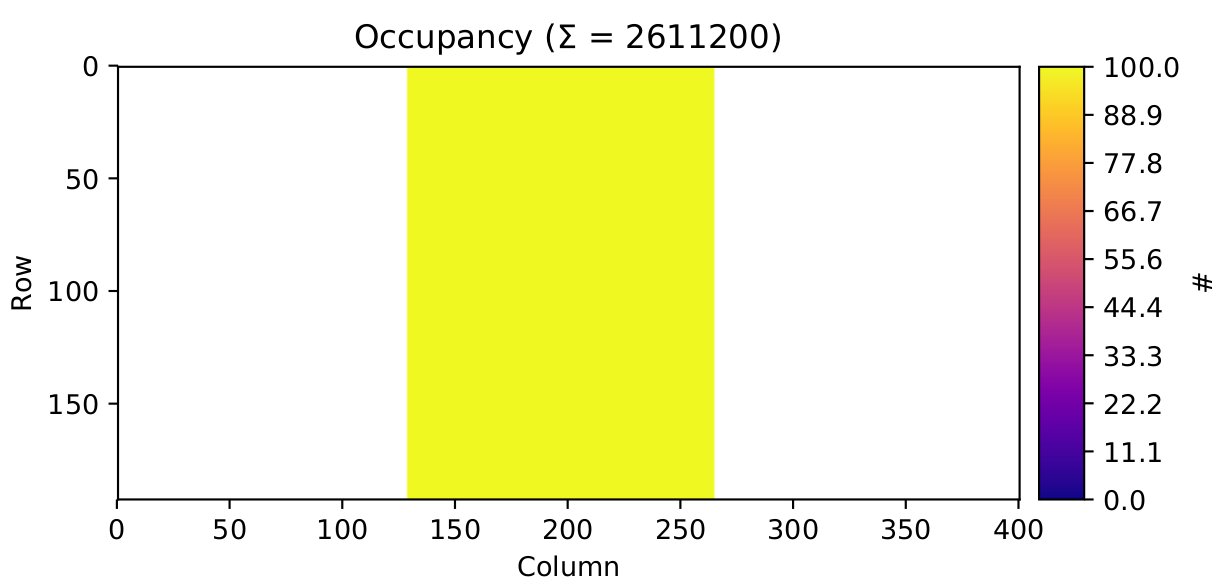
\includegraphics[width=\textwidth]{Immagini/ScanAnalogLinear}
\caption{Risultato del test \textbf{scan$\_$analog} sulla \textit{front end} lineare, tutti i canali di lettura hanno risposto il 100$\%$ delle volte.}
\label{ScanAnalogLinear}
\end{figure}
\item \textbf{scan$\_$analog} Analogo di scan$\_$digital, ma per la parte analogica: un impulso con carica specifica viene iniettato nei canali di lettura abilitati in modo da verificare il funzionamento dei \textit{front end} analogici. Un esempio è mostrato in figura \ref{ScanAnalogLinear}. %This basic scan injects a specified charge into enabled pixels to test the analog front-end. 
\item \textbf{scan$\_$threshold} Trova la soglia effettiva di ogni canale abilitato iniettando segnali con carica via via crescente.%This script scans over different amounts of injected charge to find the effective threshold of the enabled pixels.
\item \textbf{meta$\_$tune$\_$threshold$\_$simple} Scan fine delle soglie locali utilizzando, canale per canale, un DAC (\textit{Digital to Analog Converter}) a 4 bit per la sua regolazione. Il valore nella configurazione base è di 7.
  Alla fine del processo il valore di \textit{default} di ogni singolo DAC è sovrascritto da quello ottimale trovato.
%Il risultato di questo processo è un mask file.%This meta script simply performs a threshold scan for every possible TDAC to obtainthe optimal value per pixel to get as close to the target threshold as possible. The result is a TDAC mask file.
\end{itemize}
Questi script sono eseguiti girando degli script in python che leggono i parametri di configurazione dei registri contenuti nel file \textbf{default$\_$chip.yaml} scrivendoli nel chip.
%Altro file importante è il file contenente i parametri di configurazione dei registri \textbf{default$\_$chip.yaml}, che ogni volta che uno scan viene lanciato vengono scritti nel chip. 

Questi test, anche in assenza del sensore collegato al chip, permettono di: controllare separatamente le funzionalità di parte analogica e digitale separatamente; analizzare la risposta dei tre \textit{front end} ad un segnale di calibrazione; ricavare la distribuzione delle soglie, e del rumore e ottimizzare localmente le soglie (per \textit{front end} lineare e differenziale). 
% RIPARTIRE DA QUI
%Attraverso questi test è possibile, anche senza aver collegato un sensore al chip, controllare le funzionalità di parte analogica e digitale separatamente, analizzare la risposta dei tre \textit{front end} ad un segnale di calibrazione, ricavare una distribuzione delle soglie, la distribuzione del rumore e ottimizzare le soglie localmente (per \textit{front end} lineare e differenziale). 
A livello di questo lavoro di tesi risulta interessante esaminare il comportamento del circuito di alimentazione mentre il chip dialoga con il sistema di alimentazione, in presenza, quindi, di variazioni nella corrente assorbita, senza dover simulare il fenomeno dall esterno. 
Ad esempio, durante il test scan$\_$threshold, la parte analogica verifica il livello di soglia di ogni pixel andando a iniettare un segnale via via più grande nel circuito di lettura.
In questa situazione ci sono variazioni nella corrente assorbita che possono essere anche grandi. 
Come prima prova confrontiamo la differenza di comportamento del chip quando si utilizza o meno il regolatore con lo Shunt, mantenendo, comunque, sempre attiva la parte di LDO.
Andremo poi a vedere se, data la catena seriale di due chip, le attività di queste sono indipendenti o si influenzano a vicenda, i.e. se il circuito di ShuntLDO riesce a nascondere, al chip, il rumore e le eventuali fluttuazioni che vi sono nella catena.
%Una prima prova che è interessante eseguire consiste nel confrontare una situazione in cui è utilizzato il regolatore con lo Shunt e una situazione in cui non è utilizzato lo Shunt e il chip è alimentato in configurazione LDO. In seguito è lecito chiedersi se, effettivamente in una catena seriale di due chip l'attivita di uno non influenza l'altro. Cioè se il circuito di ShuntLDO riesce ad nascondere al chip eventuali fluttuazioni e rumore  che vi sono nella catena.

\subsubsection{LDOvsShuntLDO}

\begin{figure}
\centering
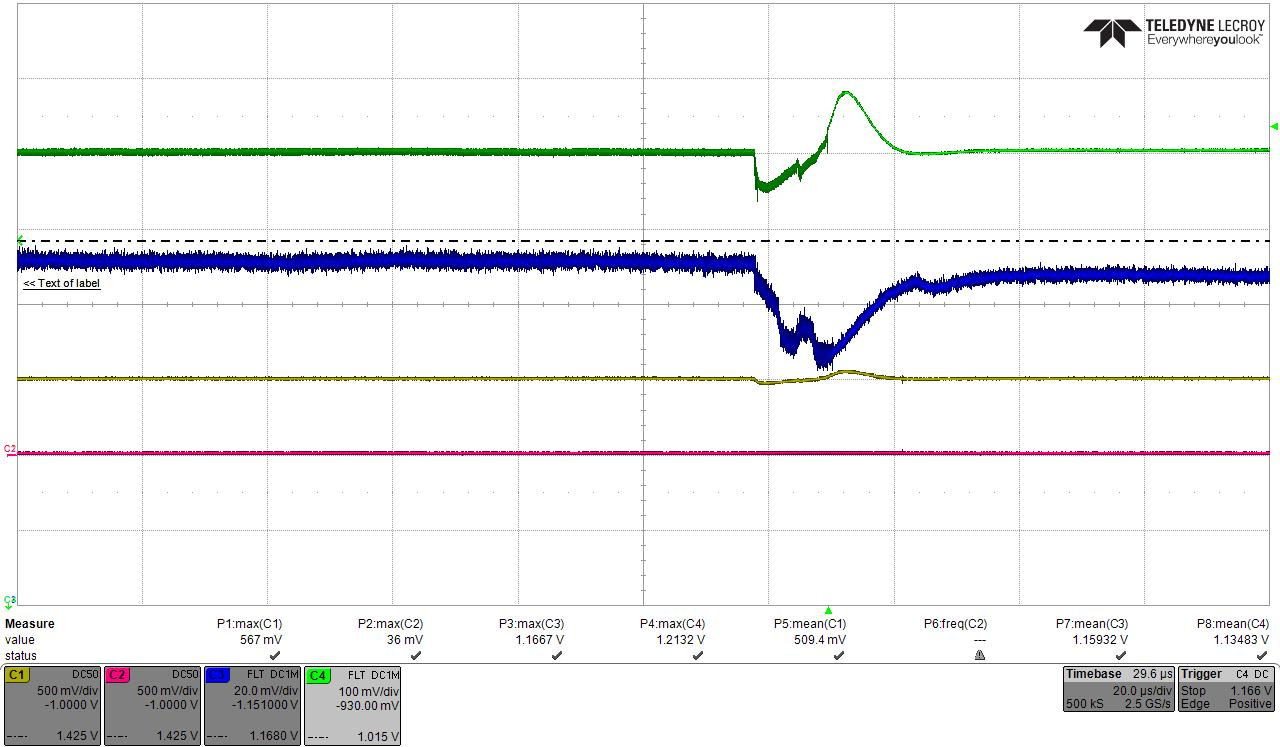
\includegraphics[scale=.3]{Immagini/alllin1}
\caption{VDDD in verde con scala 100 mV/div., e VDDA, in blu con scala 20 mV/div.}
\label{alllin1}
\end{figure}
\begin{figure}
\centering
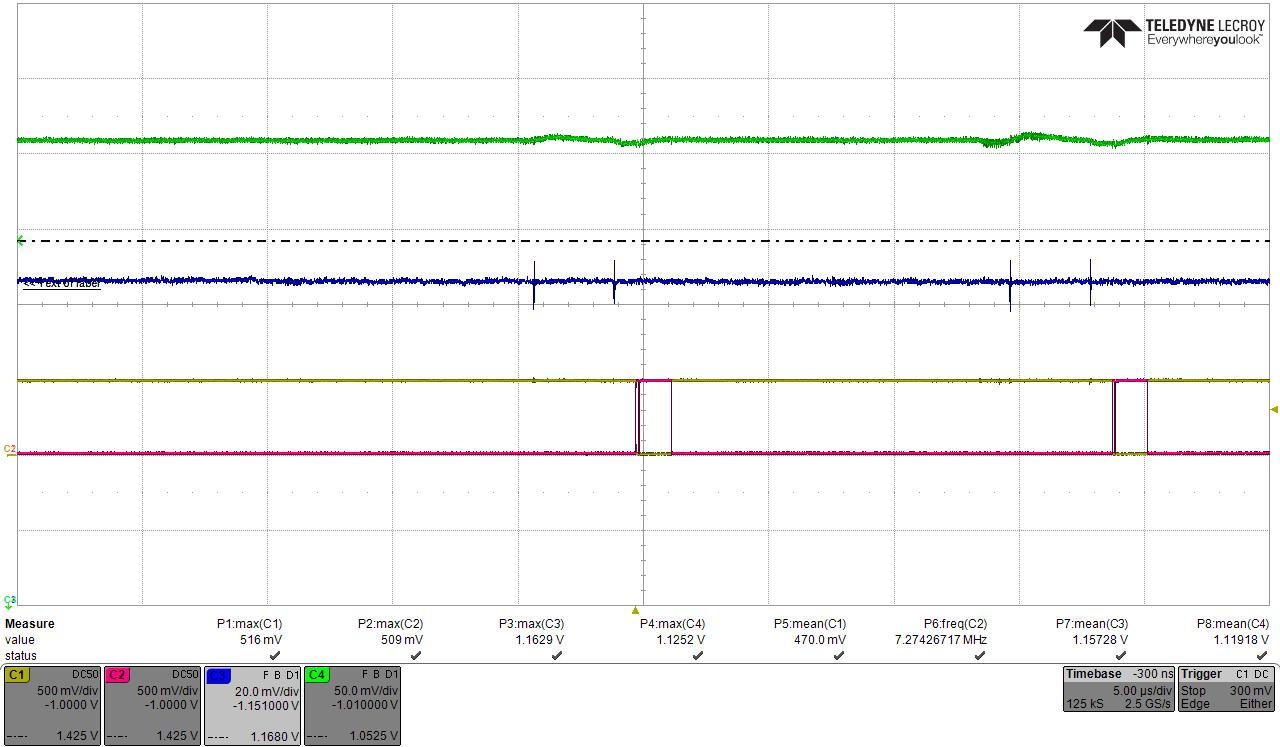
\includegraphics[scale=.3]{Immagini/alllin2}
\caption{VDDD in verde con scala 50 mV/div., e VDDA, in blu con scala 20 mV/div.}
\label{alllin2}
\end{figure}

Studiamo ora i vantaggi effettivi dell'utilizzo di un circuito di alimentazione che implementi uno Shunt oltre al regolatore.
La misura effettuata consiste nel monitorare le tensioni di alimentazione, VDDD e VDDA, mentre attraverso il sistema di acquisizione si richiede al chip di eseguire il test scan$\_$threshold
\footnote{
  Per cercare di massimizzare gli effetti è stato aumentato il numero di pixel in cui viene iniettato contemporaneamente un segnale molto grande.
}.
In questo modo è stato possibile verificare gli effetti causati dalle variazioni di carico proprie dell'attività del chip.
Dal confronto tra i risultati ottenuti in configurazione con o senza shunt è emersa chiaramente l'importanza di questo elemento, non solo per evitare che un malfunzionamento del chip renda inutilizzabile tutta la catena, ma anche per rendere stabili le tensioni generate dal regolatore. 
In figura \ref{alllin1} sono riportate le tensioni VDDD e VDDA utilizzando il chip senza Shunt (alimentato in tensione).
Durante il dialogo con il sistema di acquisizione si sono verificate variazioni notevoli nelle tensioni.
Con le stessse condizioni, ma utilizzando lo shunt, gli sbalzi di tensione, come si può vedere in figura \ref{alllin2}, spariscono poiché le variazioni di carico sono gestite localmente.
In modalità LDO, invece, l'alimentazione è in tensione ed è il generatore esterno ad adattare la corrente erogata ai consumi del chip.

%\begin{figure}
%\centering
%\includegraphics[scale=.3]{Immagini/}
%\caption{.}
%\label{}
%\end{figure}

\subsubsection{BDAQ}

\begin{figure}
\centering
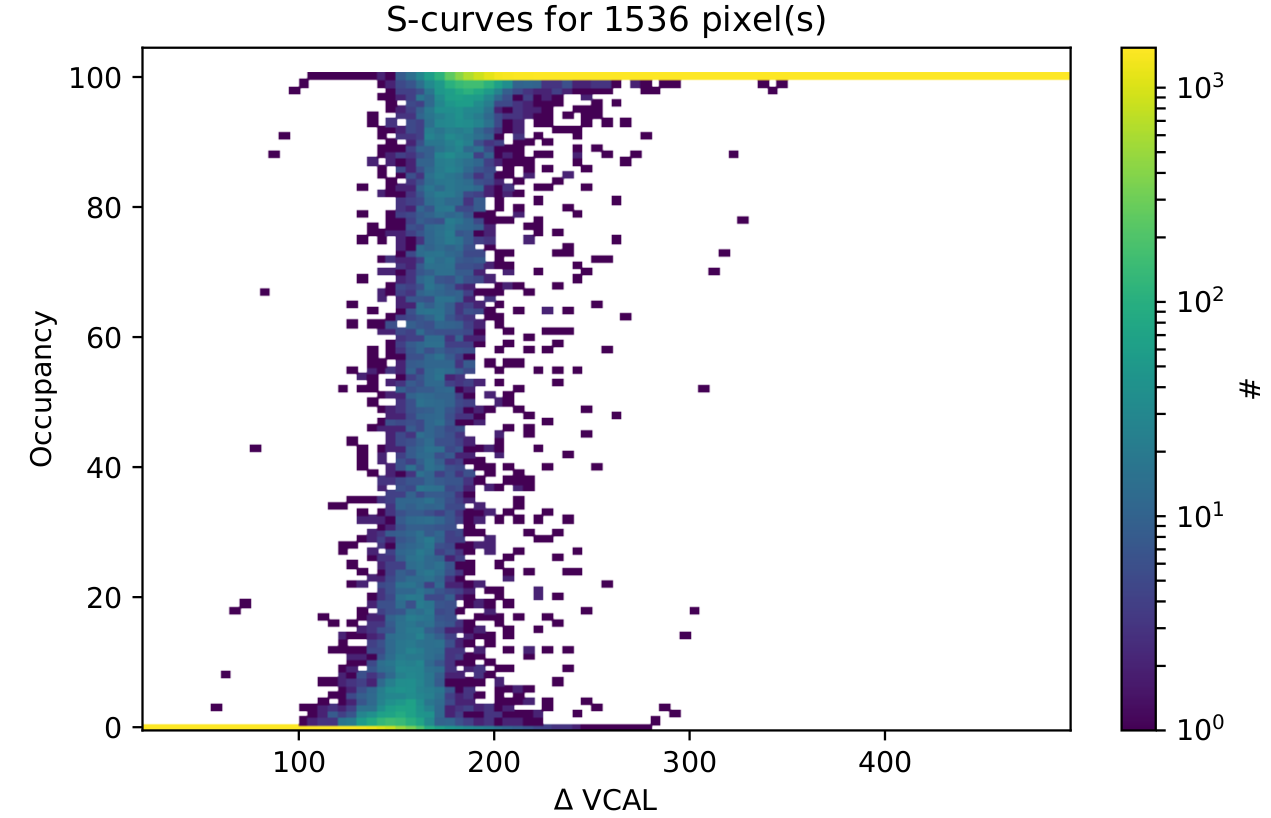
\includegraphics[width=0.9\textwidth]{Immagini/Scurves}
\caption{Risultato del test \textbf{scan$\_$threshold}. Sulle x vi è il valore, in unità arbitrarie, dell'ampiezza del segnale iniettato nel canale di lettura, sulle y il numero di volte che si è avuto risposta e n z il numero di canali.}
\label{Scurves}
\end{figure}
\begin{figure}
\centering
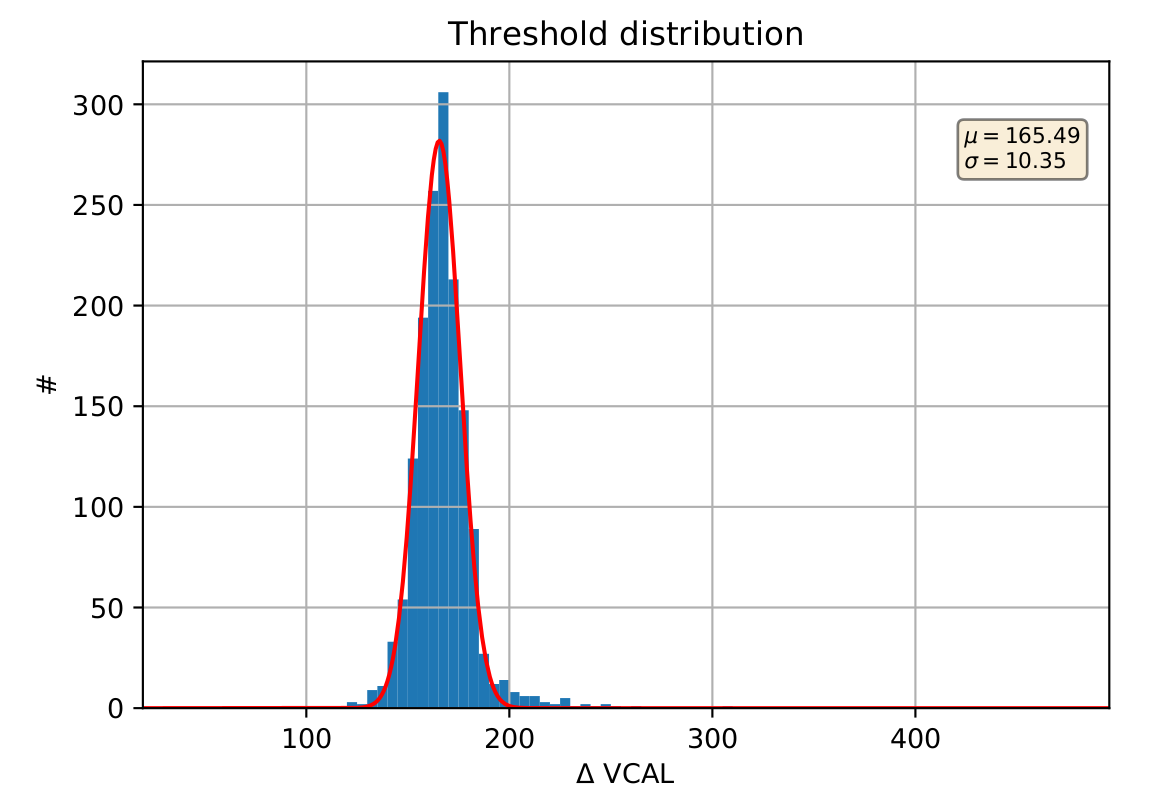
\includegraphics[width=0.75\textwidth]{Immagini/Threshold}
\caption{Distribuzione della soglia ottenuta dalle S-curves.}
\label{Threshold}
\end{figure}

%Prima di procedere con la presentazione dei risultati è necessario dare almento un'idea guida di che operazione vengono eseguite durante lo scan delle soglie al fine di comprendere meglio il significato delle varie distribuzioni.
Lo scan delle soglie, descritto all'inizio del paragrafo, permette, attraverso i parametri di configurazione, di decidere una soglia globale, uguale per tutti i canali di lettura, che nella pratica, però, varierà leggermente tra un canale e l'altro. 
%Attraverso i parametri di configurazione è possibile decidere una soglia globale uguale per tutti i canali di lettura, nella pratica però la soglia varierà leggermente tra un canale e l'altro. 
Ci si aspetta, quindi, una distribuzione delle soglie intorno ad un valore centrale.
Inoltre, a causa del rumore, la risposta del circuito di lettura in funzione della carica raccolta non sarà una theta: il rumore, che si somma al segnale, può far scattare il discriminatore anche a segnali più piccoli della soglia.
Se su ciascun canale iniettiamo un segnale sempre più grande, ripetendo il processo più volte e riportando il numero delle volte in cui il discriminatore scatta in funzione del segnale iniettato, si ottengono le così dette Scurves che, senza rumore, sarebbero a gradino. 
Mettendo insieme le Scurve di ogni canale, si ottiene un grafico come quello riportato in figura \ref{Scurves}, dove in z si ha il numero di pixel che, a un dato Vcal (in x), si sono accesi un certo numero di volte (in y).
Dal fit di ogni singola Scurve è possibile ottenere il valore di soglia e di rumore di ogni canale.
Infatti la Scurve è descritta dalla funzione:
\begin{equation}
  \mathrm{S_{curve} = \frac{A}{2} \left( 1 + \erf \left( \frac{q-\mu}{\sqrt{2}\sigma} \right) \right)},
\end{equation}
dove A è l'ampiezza della $\erf$, $\mu$ la soglia e $\sigma$ il rumore.
I valori di $\mu$ e $\sigma$ sono ricavati con il metodo descritto in \cite{ERF}.
La figura \ref{Threshold} riporta la distribuzione delle soglie dei canali con sovrapposto il fit di una gaussiana.
%Dal fit della singola Scurves si ricava un valore di soglia e rumore, mettendo insieme i risultati per tutti i canali si ottengolo le distribuzioni delle stesse, in figura\ref{Threshold} è riportata la distribuzione delle soglie. 
\begin{figure}
\centering
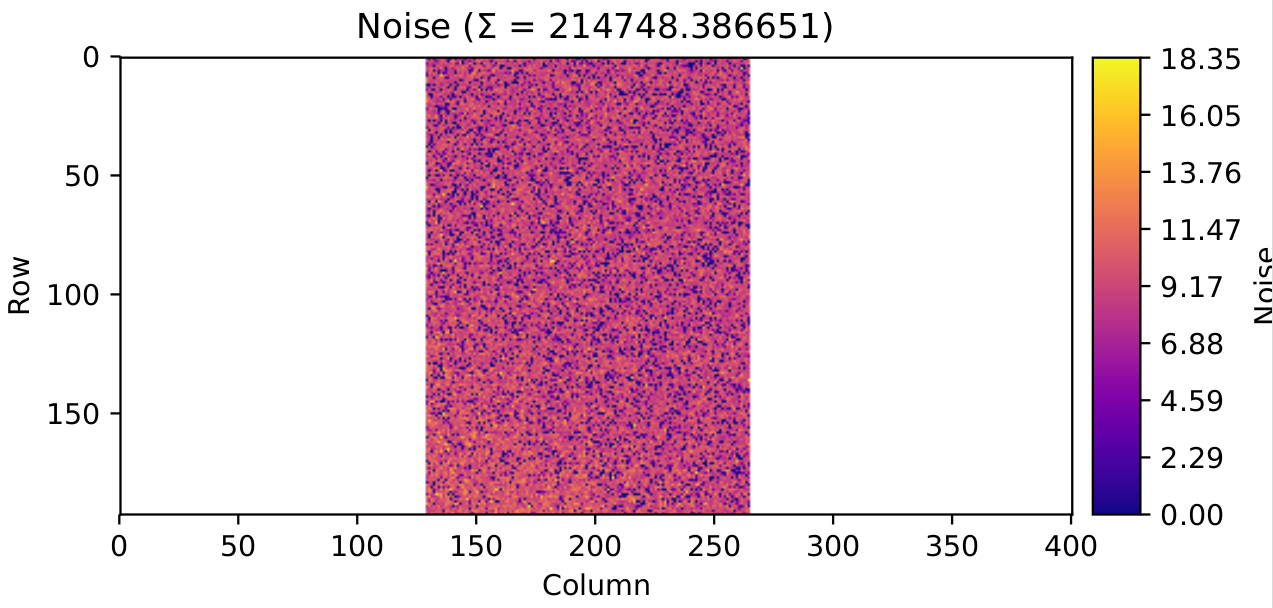
\includegraphics[width=0.9\textwidth]{Immagini/NoiseMap}
\caption{Mappa del livello di rumore pixel per pixel del FE lineare.}
\label{NoiseMap}
\end{figure}
Il test restituisce, oltre alle distribuzioni, anche le mappe di soglie e rumore utili per verificare l'omogeneità della risposta e la presenza di zone più rumorose o a rumore nullo, sintomatiche di problemi.
La figura \ref{NoiseMap} riporta la mappa del rumore ottenuta per il \textit{front end} lineare. 
%La soglia è il livello minimo a cui l'elettronica risponde, se non ci fosse rumore le S-curves sarebbero gradini, nella realtà a causa del rumore che si somma al segnale questi gradini ideali diventano curve, meno assomiglia ad un gradino maggiore è il rumore.
Come detto in precedenza l'utilizzo dello ShuntLDO dovrebbe evitare il propagarsi del rumore tra parte analogica e digitale ed evitare che disturbi della linea vengano visti dal carico. 
\begin{figure}
\centering
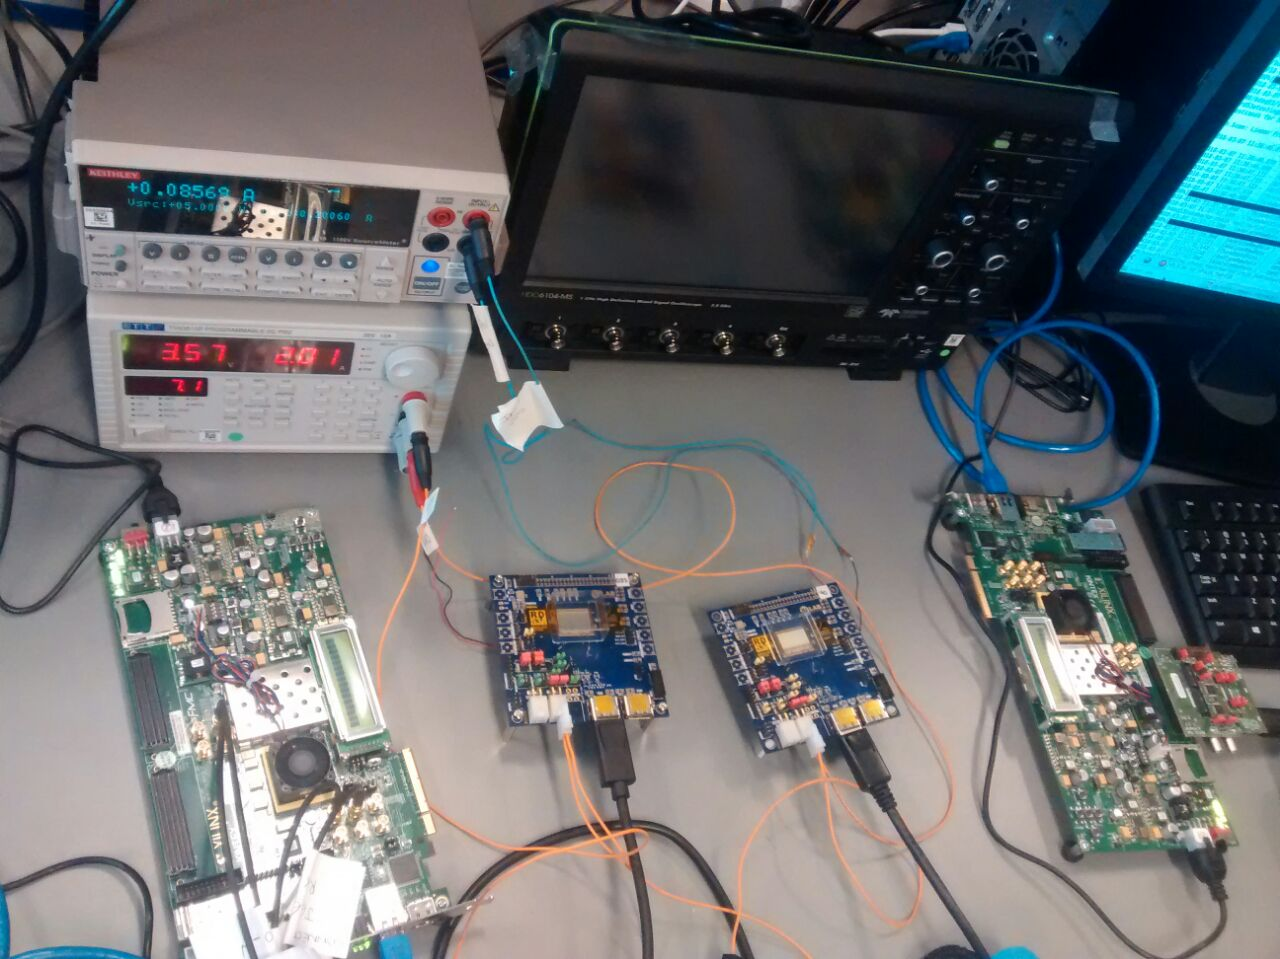
\includegraphics[width=0.75\textwidth]{Immagini/chipserial}
\caption{Fotografia del setup, i due chip posti sulla Single Chip Card sono al centro e ognuno di essi è collegato a una fpga che gestisce la comunicazione tra RD53A e il computer.}
\label{chipserial}
\end{figure}
Al fine di verificare se c'è una correlazione tra la ditribuzione del rumore e l'utilizzo del chip all'interno di una catena seriale, si sono messi a confronto i risultati ottenuti da test eseguiti con il chip singolo con quelli ottenuti poi mettendone due in serie o in parallelo, usando il setup mostrato in figura \ref{chipserial}.
Tutte e tre le misure sono state eseguite utilizzando la configurazione di ShuntLDO. 

Le misure riportate fanno riferimento solo al \textit{front end} lineare, in quanto, al momento della presa dati, era l'unico con una versione avanzata e stabile del software e con i vari parametri ben definiti.
I risulati sono riportati in funzione di VCAL, parametro dello scan, la cui conversione in elettroni è 1:10, ossia per una u.a. corrispondono 10 $\mathrm{e^{-}}$.

\begin{figure}[h]
\centering
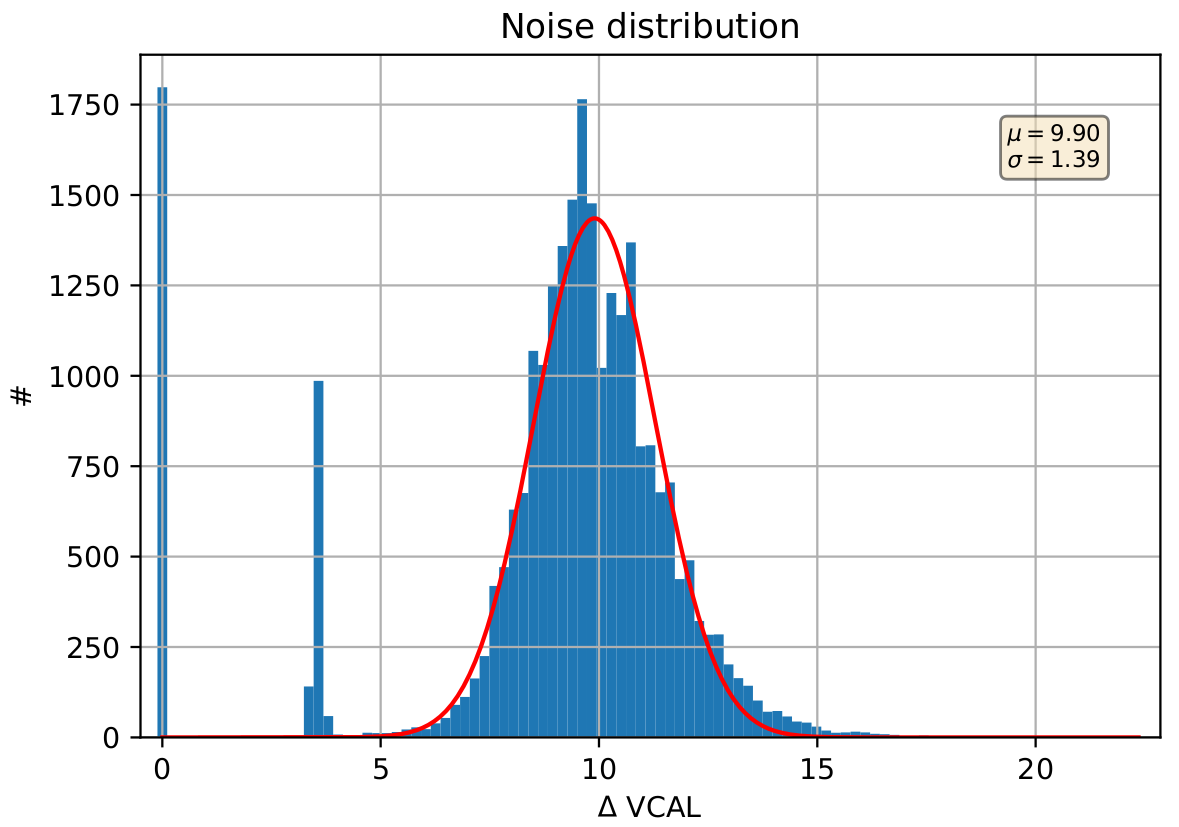
\includegraphics[width=0.75\textwidth]{Immagini/NoiseSingle}
\caption{Distribuzione di rumore ottenuta attraverso il test di \textbf{scan$\_$threshold} su un chip alimentato singolarmente.}
\label{noisesingle}
\end{figure}
\begin{figure}
\centering
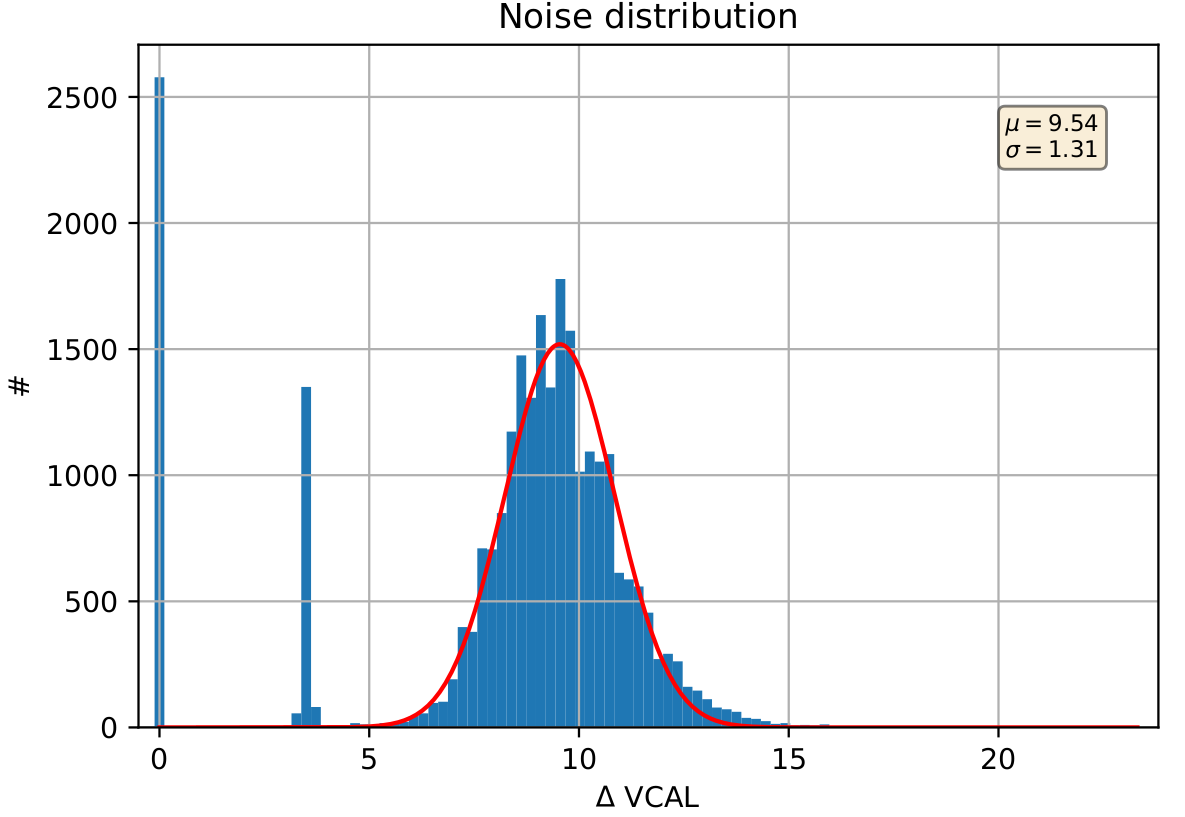
\includegraphics[width=0.75\textwidth]{Immagini/NoiseSerial}
\caption{Distribuzione di rumore ottenuta attraverso il test di \textbf{scan$\_$threshold} su un chip alimentato in serie ad un secondo, anche sul secondo chip sono stati eseguite scansioni in contemporanea.}
\label{noiseserial}
\end{figure}

Trascurando i risultati relativi alla distribuzione delle soglie, che sono indipendenti dalla distribuzione del rumore, riportiamo in figura le distribuzioni ottenute per il rumore nei tre casi:
\begin{itemize}
\item Chip singolo, figura \ref{noisesingle}.
\item Serie di due chip, figura \ref{noiseserial}.
\item Parallelo di due chip, figura \ref{noiseparallel}.
\end{itemize}
Come si può vedere, nonostante sul secondo chip fossero eseguiti test, in modo da simulare un'attività, le distribuzioni del rumore dei setup in serie e in parallelo non peggiorano rispetto al caso con con chip singolo.
Questo dimostra che, effettivamente, esternamente i chip non sono visibili e, viceversa, il chip non vede le variazioni present presentii sulla linea.

\begin{figure}
\centering
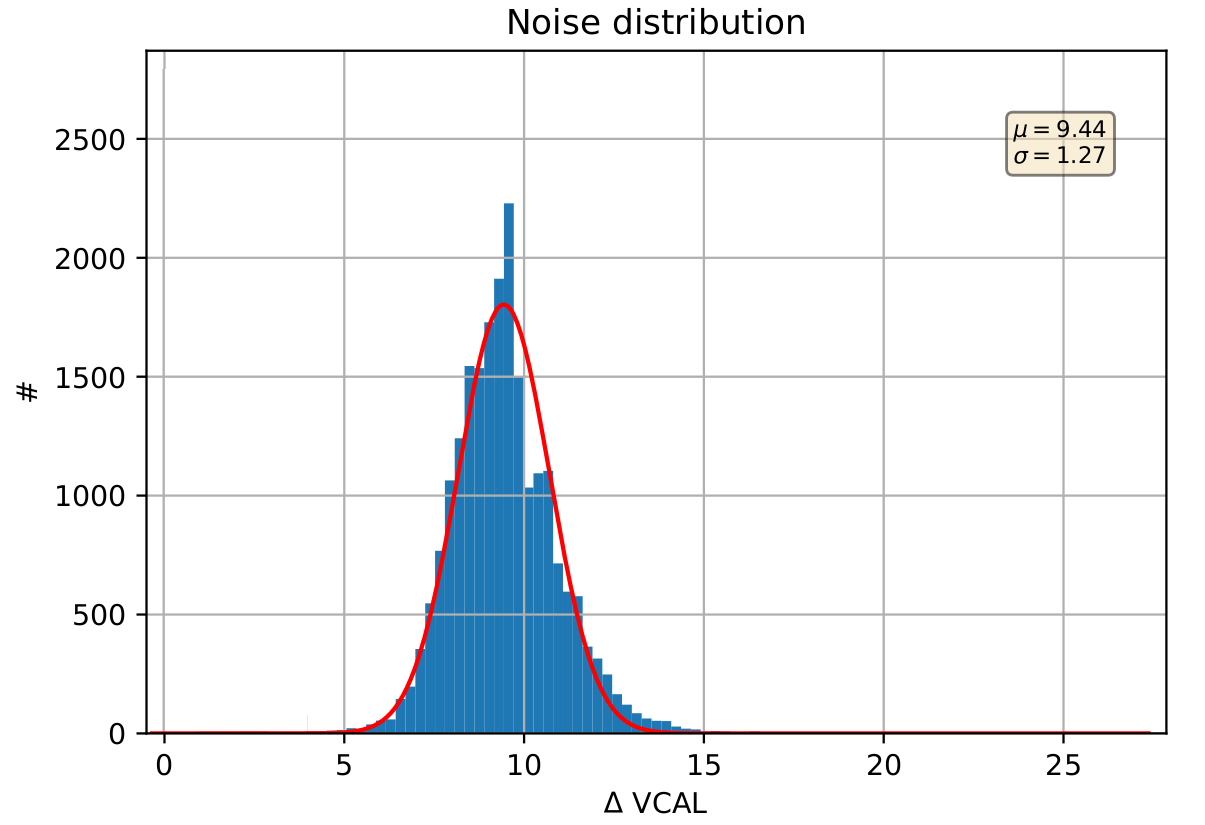
\includegraphics[width=0.75\textwidth]{Immagini/NoiseParallel}
\caption{Distribuzione di rumore ottenuta attraverso il test di \textbf{scan$\_$threshold} su un chip alimentato in parallelo ad un secondo, anche sul secondo chip sono stati eseguite scansioni in contemporanea.}
\label{noiseparallel}
\end{figure}
